%% bare_jrnl.texf
%% V1.4b
%% 2015/08/26
%% by Michael Shell
%% see http://www.michaelshell/
%% for current contact information.
%% 
%% This is a skeleton file demonstrating the use of IEEEtran.cls
%% (requires IEEEtran.cls version 1.8b or later) with an IEEE
%% journal paper.
%%
%% Support sites:
%% http://www.michaelshell.org/tex/ie eetran/
%% http://www.ctan.org/pkg/ieeetran
%% and 
%% http://www.ieee.org/

%%*************************************************************************
%% Legal Notice:
%% This code is offered as-is without any warranty either expressed or
%% implied; without even the implied warranty of MERCHANTABILITY or
%% FITNESS FOR A PARTICULAR PURPOSE! 
%% User assumes all risk.
%% In no event shall the IEEE or any contributor to this code be liable for
%% any damages or losses, including, but not limited to, incidental,
%% consequential, or any other damages, resulting from the use or misuse
%% of any information contained here.
%%
%% All comments are the opinions of their respective authors and are not
%% necessarily endorsed by the IEEE.
%%
%% This work is distributed under the LaTeX Project Public License (LPPL)
%% ( http://www.latex-project.org/ ) version 1.3, and may be freely used,
%% distributed and modified. A copy of the LPPL, version 1.3, is included
%% in the base LaTeX documentation of all distributions of LaTeX released
%% 2003/12/01 or later.
%% Retain all contribution notices and credits.
%% ** Modified files should be clearly indicated as such, including  **
%% ** renaming them and changing author support contact information. **
%%*************************************************************************


% *** Authors should verify (and, if needed, correct) their LaTeX system  ***
% *** with the testflow diagnostic prior to trusting their LaTeX platform ***
% *** with production work. The IEEE's font choices and paper sizes can   ***
% *** trigger bugs that do not appear when using other class files.       ***                          ***
% The testflow support page is at:
% http://www.michaelshell.org/tex/testflow/



\documentclass[journal]{IEEEtran}

%
% If IEEEtran.cls has not been installed into the LaTeX system files,
% manually specify the path to it like:
% \documentclass[journal]{../sty/IEEEtran}





% Some very useful LaTeX packages include:
% (uncomment the ones you want to load)


% *** MISC UTILITY PACKAGES ***
%
%\usepackage{ifpdf}
% Heiko Oberdiek's ifpdf.sty is very useful if you need conditional
% compilation based on whether the output is pdf or dvi.
% usage:
% \ifpdf
%   % pdf code
% \else
%   % dvi code
% \fi
% The latest version of ifpdf.sty can be obtained from:
% http://www.ctan.org/pkg/ifpdf
% Also, note that IEEEtran.cls V1.7 and later provides a builtin
% \ifCLASSINFOpdf conditional that works the same way.
% When switching from latex to pdflatex and vice-versa, the compiler may
% have to be run twice to clear warning/error messages.






% *** CITATION PACKAGES ***
%
\usepackage{cite}
% cite.sty was written by Donald Arseneau
% V1.6 and later of IEEEtran pre-defines the format of the cite.sty package
% \cite{} output to follow that of the IEEE. Loading the cite package will
% result in citation numbers being automatically sorted and properly
% "compressed/ranged". e.g., [1], [9], [2], [7], [5], [6] without using
% cite.sty will become [1], [2], [5]--[7], [9] using cite.sty. cite.sty's
% \cite will automatically add leading space, if needed. Use cite.sty's
% noadjust option (cite.sty V3.8 and later) if you want to turn this off
% such as if a citation ever needs to be enclosed in parenthesis.
% cite.sty is already installed on most LaTeX systems. Be sure and use
% version 5.0 (2009-03-20) and later if using hyperref.sty.
% The latest version can be obtained at:
% http://www.ctan.org/pkg/cite
% The documentation is contained in the cite.sty file itself.






% *** GRAPHICS RELATED PACKAGES ***
%
\ifCLASSINFOpdf
  \usepackage[pdftex]{graphicx}
  % declare the path(s) where your graphic files are
  % \graphicspath{{../pdf/}{../jpeg/}}
  % and their extensions so you won't have to specify these with
  % every instance of \includegraphics
  % \DeclareGraphicsExtensions{.pdf,.jpeg,.png}
\else
  % or other class option (dvipsone, dvipdf, if not using dvips). graphicx
  % will default to the driver specified in the system graphics.cfg if no
  % driver is specified.
  % \usepackage[dvips]{graphicx}
  % declare the path(s) where your graphic files are
  % \graphicspath{{../eps/}}
  % and their extensions so you won't have to specify these with
  % every instance of \includegraphics
  % \DeclareGraphicsExtensions{.eps}
\fi
% graphicx was written by David Carlisle and Sebastian Rahtz. It is
% required if you want graphics, photos, etc. graphicx.sty is already
% installed on most LaTeX systems. The latest version and documentation
% can be obtained at: 
% http://www.ctan.org/pkg/graphicx
% Another good source of documentation is "Using Imported Graphics in
% LaTeX2e" by Keith Reckdahl which can be found at:
% http://www.ctan.org/pkg/epslatex
%
% latex, and pdflatex in dvi mode, support graphics in encapsulated
% postscript (.eps) format. pdflatex in pdf mode supports graphics
% in .pdf, .jpeg, .png and .mps (metapost) formats. Users should ensure
% that all non-photo figures use a vector format (.eps, .pdf, .mps) and
% not a bitmapped formats (.jpeg, .png). The IEEE frowns on bitmapped formats
% which can result in "jaggedy"/blurry rendering of lines and letters as
% well as large increases in file sizes.
%
% You can find documentation about the pdfTeX application at:
% http://www.tug.org/applications/pdftex





% *** MATH PACKAGES ***
%
\usepackage{amsmath}
% A popular package from the American Mathematical Society that provides
% many useful and powerful commands for dealing with mathematics.
%
% Note that the amsmath package sets \interdisplaylinepenalty to 10000
% thus preventing page breaks from occurring within multiline equations. Use:
\interdisplaylinepenalty=2500
% after loading amsmath to restore such page breaks as IEEEtran.cls normally
% does. amsmath.sty is already installed on most LaTeX systems. The latest
% version and documentation can be obtained at:
% http://www.ctan.org/pkg/amsmath





% *** SPECIALIZED LIST PACKAGES ***
%
%\usepackage{algorithmic}
% algorithmic.sty was written by Peter Williams and Rogerio Brito.
% This package provides an algorithmic environment fo describing algorithms.
% You can use the algorithmic environment in-text or within a figure
% environment to provide for a floating algorithm. Do NOT use the algorithm
% floating environment provided by algorithm.sty (by the same authors) or
% algorithm2e.sty (by Christophe Fiorio) as the IEEE does not use dedicated
% algorithm float types and packages that provide these will not provide
% correct IEEE style captions. The latest version and documentation of
% algorithmic.sty can be obtained at:
% http://www.ctan.org/pkg/algorithms
% Also of interest may be the (relatively newer and more customizable)
% algorithmicx.sty package by Szasz Janos:
% http://www.ctan.org/pkg/algorithmicx




% *** ALIGNMENT PACKAGES ***
%
\usepackage{array}
% Frank Mittelbach's and David Carlisle's array.sty patches and improves
% the standard LaTeX2e array and tabular environments to provide better
% appearance and additional user controls. As the default LaTeX2e table
% generation code is lacking to the point of almost being broken with
% respect to the quality of the end results, all users are strongly
% advised to use an enhanced (at the very least that provided by array.sty)
% set of table tools. array.sty is already installed on most systems. The
% latest version and documentation can be obtained at:
% http://www.ctan.org/pkg/array


% IEEEtran contains the IEEEeqnarray family of commands that can be used to
% generate multiline equations as well as matrices, tables, etc., of high
% quality.




% *** SUBFIGURE PACKAGES ***
\ifCLASSOPTIONcompsoc
  \usepackage[caption=false,font=normalsize,labelfont=sf,textfont=sf]{subfig}
\else
\usepackage[caption=false,font=footnotesize]{subfig}
\fi
% subfig.sty, written by Steven Douglas Cochran, is the modern replacement
% for subfigure.sty, the latter of which is no longer maintained and is
% incompatible with some LaTeX packages including fixltx2e. However,
% subfig.sty requires and automatically loads Axel Sommerfeldt's caption.sty
% which will override IEEEtran.cls' handling of captions and this will result
% in non-IEEE style figure/table captions. To prevent this problem, be sure
% and invoke subfig.sty's "caption=false" package option (available since
% subfig.sty version 1.3, 2005/06/28) as this is will preserve IEEEtran.cls
% handling of captions.
% Note that the Computer Society format requires a larger sans serif font
% than the serif footnote size font used in traditional IEEE formatting
% and thus the need to invoke different subfig.sty package options depending
% on whether compsoc mode has been enabled.
%
% The latest version and documentation of subfig.sty can be obtained at:
% http://www.ctan.org/pkg/subfig




% *** FLOAT PACKAGES ***
%
%\usepackage{fixltx2e}
% fixltx2e, the successor to the earlier fix2col.sty, was written by
% Frank Mittelbach and David Carlisle. This package corrects a few problems
% in the LaTeX2e kernel, the most notable of which is that in current
% LaTeX2e releases, the ordering of single and double column floats is not
% guaranteed to be preserved. Thus, an unpatched LaTeX2e can allow a
% single column figure to be placed prior to an earlier double column
% figure.
% Be aware that LaTeX2e kernels dated 2015 and later have fixltx2e.sty's
% corrections already built into the system in which case a warning will
% be issued if an attempt is made to load fixltx2e.sty as it is no longer
% needed.
% The latest version and documentation can be found at:
% http://www.ctan.org/pkg/fixltx2e


%\usepackage{stfloats}
% stfloats.sty was written by Sigitas Tolusis. This package gives LaTeX2e
% the ability to do double column floats at the bottom of the page as well
% as the top. (e.g., "\begin{figure*}[!b]" is not normally possible in
% LaTeX2e). It also provides a command:
%\fnbelowfloat
% to enable the placement of footnotes below bottom floats (the standard
% LaTeX2e kernel puts them above bottom floats). This is an invasive package
% which rewrites many portions of the LaTeX2e float routines. It may not work
% with other packages that modify the LaTeX2e float routines. The latest
% version and documentation can be obtained at:
% http://www.ctan.org/pkg/stfloats
% Do not use the stfloats baselinefloat ability as the IEEE does not allow
% \baselineskip to stretch. Authors submitting work to the IEEE should note
% that the IEEE rarely uses double column equations and that authors should try
% to avoid such use. Do not be tempted to use the cuted.sty or midfloat.sty
% packages (also by Sigitas Tolusis) as the IEEE does not format its papers in
% such ways.
% Do not attempt to use stfloats with fixltx2e as they are incompatible.
% Instead, use Morten Hogholm'a dblfloatfix which combines the features
% of both fixltx2e and stfloats:
%
% \usepackage{dblfloatfix}
% The latest version can be found at:
% http://www.ctan.org/pkg/dblfloatfix




%\ifCLASSOPTIONcaptionsoff
%  \usepackage[nomarkers]{endfloat}
% \let\MYoriglatexcaption\caption
% \renewcommand{\caption}[2][\relax]{\MYoriglatexcaption[#2]{#2}}
%\fi
% endfloat.sty was written by James Darrell McCauley, Jeff Goldberg and 
% Axel Sommerfeldt. This package may be useful when used in conjunction with 
% IEEEtran.cls'  captionsoff option. Some IEEE journals/societies require that
% submissions have lists of figures/tables at the end of the paper and that
% figures/tables without any captions are placed on a page by themselves at
% the end of the document. If needed, the draftcls IEEEtran class option or
% \CLASSINPUTbaselinestretch interface can be used to increase the line
% spacing as well. Be sure and use the nomarkers option of endfloat to
% prevent endfloat from "marking" where the figures would have been placed
% in the text. The two hack lines of code above are a slight modification of
% that suggested by in the endfloat docs (section 8.4.1) to ensure that
% the full captions always appear in the list of figures/tables - even if
% the user used the short optional argument of \caption[]{}.
% IEEE papers do not typically make use of \caption[]'s optional argument,
% so this should not be an issue. A similar trick can be used to disable
% captions of packages such as subfig.sty that lack options to turn off
% the subcaptions:
% For subfig.sty:
% \let\MYorigsubfloat\subfloat
% \renewcommand{\subfloat}[2][\relax]{\MYorigsubfloat[]{#2}}
% However, the above trick will not work if both optional arguments of
% the \subfloat command are used. Furthermore, there needs to be a
% description of each subfigure *somewhere* and endfloat does not add
% subfigure captions to its list of figures. Thus, the best approach is to
% avoid the use of subfigure captions (many IEEE journals avoid them anyway)
% and instead reference/explain all the subfigures within the main caption.
% The latest version of endfloat.sty and its documentation can obtained at:
% http://www.ctan.org/pkg/endfloat
%
% The IEEEtran \ifCLASSOPTIONcaptionsoff conditional can also be used
% later in the document, say, to conditionally put the References on a 
% page by themselves.




% *** PDF, URL AND HYPERLINK PACKAGES ***
%
\usepackage{url}
% url.sty was written by Donald Arseneau. It provides better support for
% handling and breaking URLs. url.sty is already installed on most LaTeX
% systems. The latest version and documentation can be obtained at:
% http://www.ctan.org/pkg/url
% Basically, \url{my_url_here}.




% *** Do not adjust lengths that control margins, column widths, etc. ***
% *** Do not use packages that alter fonts (such as pslatex).         ***
% There should be no need to do such things with IEEEtran.cls V1.6 and later.
% (Unless specifically asked to do so by the journal or conference you plan
% to submit to, of course. )


%%%%%%%%%%%%%%%%%%%%%%%%%%% AUTHOR'S HEADER %%%%%%%%%%%%%%%%%%%%%%%%%%%%%%%%
\usepackage{xspace}
\newcommand*{\eg}{e.g.\@\xspace}
\newcommand*{\etc}{etc.\@\xspace}
\newcommand*{\ie}{i.e.\@\xspace}
\newcommand*{\resp}{resp.\@\xspace}
\newcommand*{\vs}{vs.\@\xspace}
\newcommand\Fscore{$F_1$-score}

\usepackage{mathptmx}
\usepackage{amsmath}
\usepackage{amssymb}
\usepackage{amsthm}
\newtheorem{thm}{Theorem}[section]
\newtheorem{lem}[thm]{Lemma}
\newtheorem{prop}[thm]{Proposition}
\newtheorem*{prop*}{Proposition}
\theoremstyle{remark}
\newtheorem*{remark}{Remark}
\renewcommand{\qedsymbol}{$\blacksquare$}
\usepackage{siunitx}
\usepackage{enumitem}
\usepackage{adjustbox}
\usepackage{stackengine}
\usepackage{url}
\urlstyle{same}
\usepackage{microtype}

% correct bad hyphenation here
\hyphenation{op-tical net-works semi-conduc-tor}

\begin{document}
%
% paper title
% Titles are generally capitalized except for words such as a, an, and, as,
% at, but, by, for, in, nor, of, on, or, the, to and up, which are usually
% not capitalized unless they are the first or last word of the title.
% Linebreaks \\ can be used within to get better formatting as desired.
% Do not put math or special symbols in the title.
\title{Per-Channel Energy Normalization: Why and How}
%
%
% author names and IEEE memberships
% note positions of commas and nonbreaking spaces ( ~ ) LaTeX will not break
% a structure at a ~ so this keeps an author's name from being broken across
% two lines.
% use \thanks{} to gain access to the first footnote area
% a separate \thanks must be used for each paragraph as LaTeX2e's \thanks
% was not built to handle multiple paragraphs
%

%\author{Michael~Shell,~\IEEEmembership{Member,~IEEE,}
%        John~Doe,~\IEEEmembership{Fellow,~OSA,}
%        and~Jane~Doe,~\IEEEmembership{Life~Fellow,~IEEE}% <-this % stops a space
%\thanks{M. Shell was with the Department
%of Electrical and Computer Engineering, Georgia Institute of Technology, Atlanta,
%GA, 30332 USA e-mail: (see http://www.michaelshell.org/contact.html).}% <-this % stops a space
%\thanks{J. Doe and J. Doe are with Anonymous University.}% <-this % stops a space
%\thanks{Manuscript received April 19, 2005; revised August 26, 2015.}}

\author{Vincent~Lostanlen, Justin~Salamon, Mark~Cartwright, Brian~McFee,\\
Andrew~Farnsworth, Steve~Kelling, and Juan~Pablo~Bello% <-this % stops a space
\thanks{V. Lostanlen, A. Farnsworth, and S. Kelling are with the Cornell Lab of Ornithology.
J. Salamon, M. Cartwright, B. McFee, and J. P. Bello are with New York University.}% <-this % stops a space
}

% note the % following the last \IEEEmembership and also \thanks - 
% these prevent an unwanted space from occurring between the last author name
% and the end of the author line. i.e., if you had this:
% 
% \author{....lastname \thanks{...} \thanks{...} }
%                     ^------------^------------^----Do not want these spaces!
%
% a space would be appended to the last name and could cause every name on that
% line to be shifted left slightly. This is one of those "LaTeX things". For
% instance, "\textbf{A} \textbf{B}" will typeset as "A B" not "AB". To get
% "AB" then you have to do: "\textbf{A}\textbf{B}"
% \thanks is no different in this regard, so shield the last } of each \thanks
% that ends a line with a % and do not let a space in before the next \thanks.
% Spaces after \IEEEmembership other than the last one are OK (and needed) as
% you are supposed to have spaces between the names. For what it is worth,
% this is a minor point as most people would not even notice if the said evil
% space somehow managed to creep in.



% The paper headers
\markboth{IEEE Signal Processing Letters, Submitted~July~2018, Accepted~September~2018, Published~November~2018}%
{Lostanlen \MakeLowercase{\textit{et al.}}: \title{}}
% The only time the second header will appear is for the odd numbered pages
% after the title page when using the twoside option.
% 
% *** Note that you probably will NOT want to include the author's ***
% *** name in the headers of peer review papers.                   ***
% You can use \ifCLASSOPTIONpeerreview for conditional compilation here if
% you desire.




% If you want to put a publisher's ID mark on the page you can do it like
% this:
%\IEEEpubid{0000--0000/00\$00.00~\copyright~2015 IEEE}
% Remember, if you use this you must call \IEEEpubidadjcol in the second
% column for its text to clear the IEEEpubid mark.



% use for special paper notices
%\IEEEspecialpapernotice{(Invited Paper)}




% make the title area
\maketitle

% As a general rule, do not put math, special symbols or citations
% in the abstract or keywords.
\begin{abstract}
In the context of automatic speech recognition and acoustic event detection, an adaptive procedure named per-channel energy normalization (PCEN) has recently shown to outperform the pointwise logarithm of mel-frequency spectrogram (logmelspec) as an acoustic frontend.
This article investigates the adequacy of PCEN for spectrogram-based pattern recognition in far-field noisy recordings, both from theoretical and practical standpoints.
First, we apply PCEN on various datasets of natural acoustic environments and find empirically that it Gaussianizes distributions of magnitudes while decorrelating frequency bands.
Secondly, we describe the asymptotic regimes of each component in PCEN: temporal integration, gain control, and dynamic range compression.
Thirdly, we give practical advice for adapting PCEN parameters to the temporal properties of the noise to be mitigated, the signal to be enhanced, and the choice of time-frequency representation.
As it converts a large class of real-world soundscapes into additive white Gaussian noise (AWGN), PCEN is a computationally efficient frontend for robust detection and classification of acoustic events in heterogeneous environments.
\end{abstract}

% Note that keywords are not normally used for peerreview papers.
\begin{IEEEkeywords}
Acoustic noise, acoustic sensors, acoustic signal detection, signal classification, spectrogram.
\end{IEEEkeywords}

% For peer review papers, you can put extra information on the cover
% page as needed:
% \ifCLASSOPTIONpeerreview
% \begin{center} \bfseries EDICS Category: 3-BBND \end{center}
% \fi
%
% For peerreview papers, this IEEEtran command inserts a page break and
% creates the second title. It will be ignored for other modes.
\IEEEpeerreviewmaketitle

\section{Introduction}
% The very first letter is a 2 line initial drop letter followed
% by the rest of the first word in caps.
% 
% form to use if the first word consists of a single letter:
% \IEEEPARstart{A}{demo} file is ....
% 
% form to use if you need the single drop letter followed by
% normal text (unknown if ever used by the IEEE):
% \IEEEPARstart{A}{}demo file is ....
% 
% Some journals put the first two words in caps:
% \IEEEPARstart{T}{his demo} file is ....
%
\IEEEPARstart{F}{requency} transposition is a major factor of intra-class variability in many sound classification tasks, including automatic speech recognition (ASR)   \cite{abdel2014taslp}, acoustic event detection (AED) \cite{espi2015eurasip}, and bioacoustic species classification \cite{salamon2017icassp}.
Tuning auditory filters to the perceptual mel scale provides a time-frequency representation, named mel-frequency spectrogram, in which the frequency transpositions of any periodic audio signal become vertical translations \cite{umesh1999icassp}.
In the presence of a single source, this property allows convolutional operators in the time-frequency domain \cite{lostanlen2017phd}, such as convolutional neural networks \cite{abdel2014taslp} and time-frequency scattering \cite{anden2015mlsp}, to extract pitch contours as spectrotemporal patterns, regardless of their fundamental frequency -- a property known as equivariance \cite{kondor2018icml,mallat2016rsta}.

Yet, there is often more than one active source in real-world audio recordings, especially outdoors \cite{mesaros2015applied}.
Even after narrowing down the classification task to the identification of the most salient source only (thereafter called foreground), the presence of background noise is detrimental to equivariance along the mel-frequency axis \cite{salamon2017spl}.
Indeed, on one hand, intra-class variability causes frequency transposition of the foreground while leaving the background unaffected.
On the other hand, equivariance is only possible if foreground and background happen to be transposed simultaneously.
%The contradiction of these two assumptions hinders generalization of learned convolutional kernels across acoustically similar events of distinct fundamental frequencies.
The generalizability of learned convolutional kernels across acoustically similar events of distinct fundamental frequencies is hindered by the contradiction between these two assumptions.
To reconcile them, the background must result from a stochastic process that is stationary along the mel-frequency axis \cite{badeau2016techreport}.
Indeed, the robustness of deep neural networks to adversarial additive perturbations has been shown to be theoretically optimal if background noise in the training set is additive, white, and Gaussian (AWGN) \cite{franceschi2018aistats}.
However, in the absence of any further processing, magnitudes in the mel-frequency spectrogram $\mathbf{E}(t, f)$ of real-world acoustic scenes are typically sparse and strongly correlated, both along time $t$ and mel frequency $f $\cite{mcdermott2011neuron}, and thus not approximable by AWGN. 
 

\begin{figure}
\centering
\subfloat[Logarithmic transformation.]{%
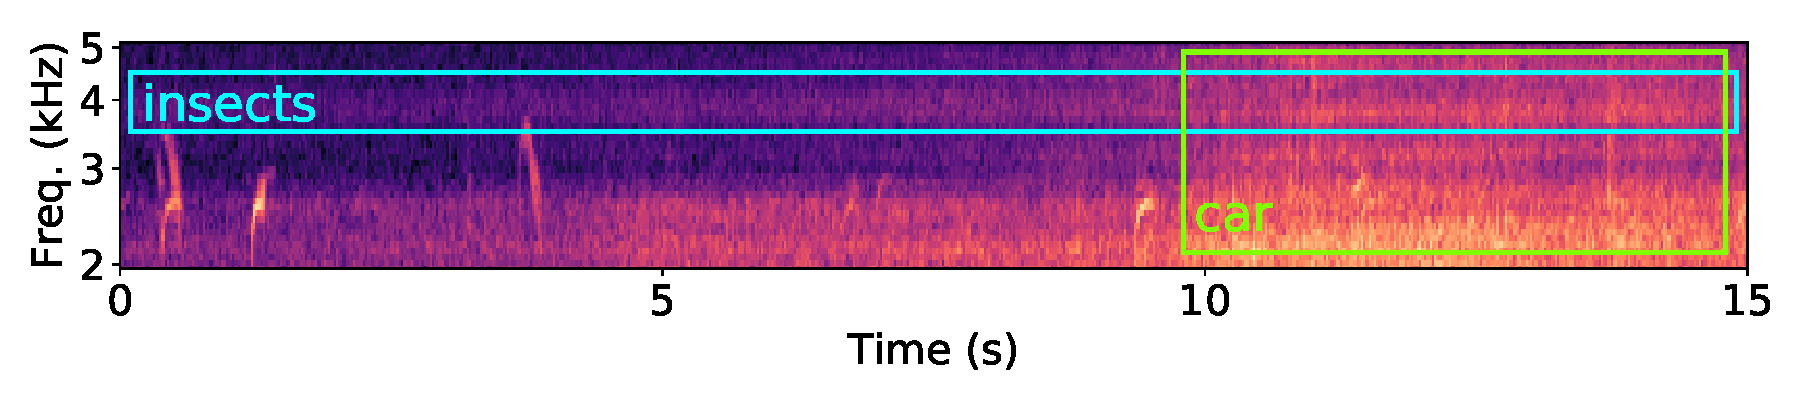
\includegraphics[width=\linewidth,keepaspectratio]{logE_spectrogram.eps}}\\
%\subfloat[Box-Cox transformation.]{ 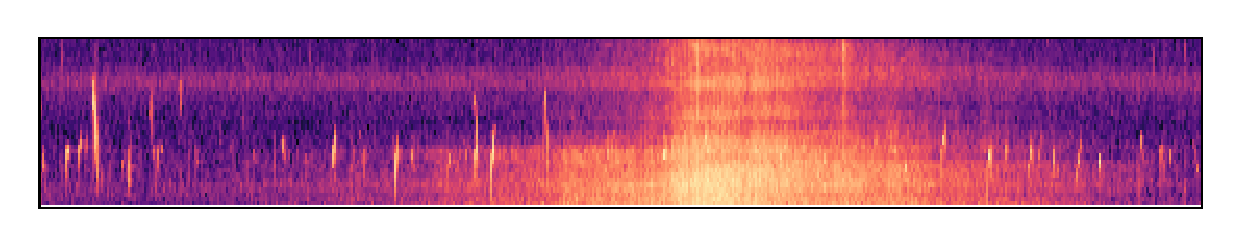
\includegraphics[width=\linewidth]{BC_spectrogram.eps}}\\
\subfloat[Per-channel energy normalization (PCEN).]{%
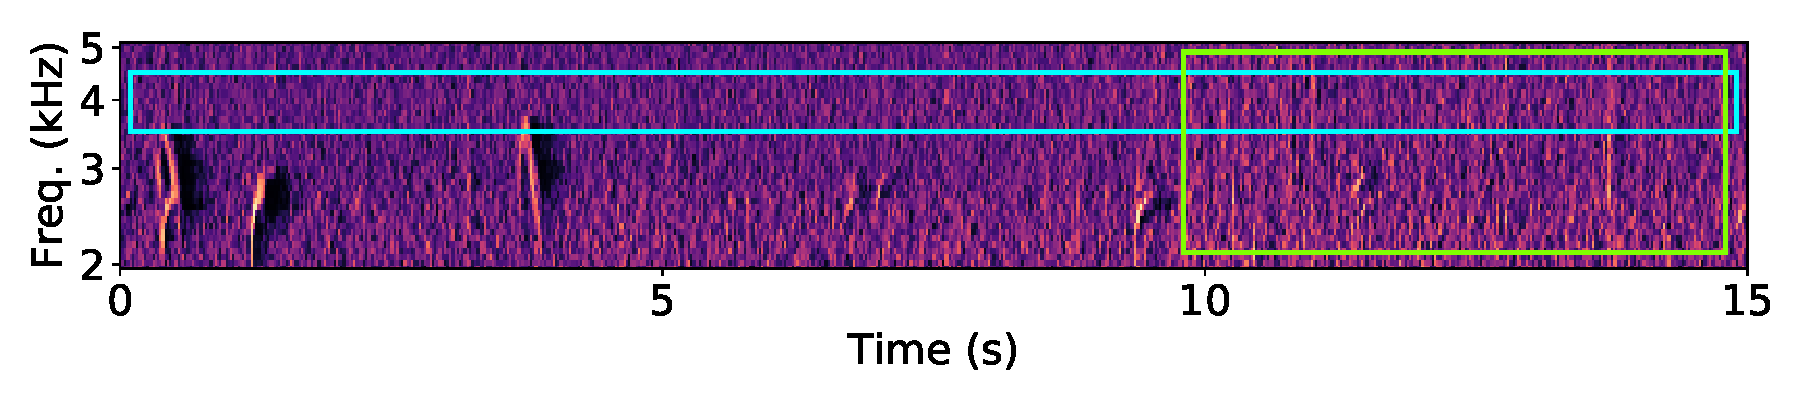
\includegraphics[width=\linewidth,keepaspectratio]{PCEN_spectrogram.eps}}
\caption{A soundscape comprising bird calls, insect stridulations, and a passing vehicle.
%, as recorded from an omnidirectional acoustic sensor.
The logarithmic transformation of the mel-frequency spectrogram (a) maps all magnitudes to a decibel-like scale, whereas per-channel energy normalization (b) enhances transient events (bird calls) while discarding stationary noise (insects) as well as slow changes in loudness (vehicle). Data provided by BirdVox. Mel-frequency spectrogram and PCEN computed with default librosa 0.6.1 parameters and $T=\SI{60}{\milli\second}$ (see Section \ref{sec:practical-recommendations}).}
\label{fig:spectrogram}
\end{figure} 

Per-channel energy normalization (PCEN) \cite{wang2017icassp} has recently been proposed as an alternative to the logarithmic transformation of the mel-frequency spectrogram (logmelspec), with the aim of improving robustness to channel distortion.
PCEN combines dynamic range compression (DRC, also present in logmelspec) and adaptive gain control (AGC) with temporal integration. AGC is a prior stage to DRC involving a low-pass filter $\mathbf{\phi}_T$ at a time scale $T$, thus yielding
\begin{equation}
\mathbf{PCEN}(t,f) =
\left(\dfrac{\mathbf{E}(t,f)}{(\varepsilon+(\mathbf{E}\overset{t}{\ast}\boldsymbol{\phi}_T)(t,f))^\alpha} + \delta\right)^r - \delta^r
\end{equation}
where $\alpha, \varepsilon, r$, and $\delta$ are positive constants.
While DRC reduces the variance of foreground loudness, AGC is intended to suppress stationary background noise.
The resulting representation has shown to improve performance in far-field ASR \cite{battenberg2017arxiv}, AED \cite{krstulovic2018casse}, keyword spotting \cite{wang2017icassp, shan2018attention}, and vocal activity detection in music \cite{schluter2018ismir}. However, the literature is yet to provide clear insight into why and how PCEN works.

This article aims to address this gap by showing empirically how PCEN Gaussianizes and whitens mel-frequency magnitude spectra in various acoustic conditions, characterizing the effect of its various parameters by means of theoretical and practical insights combined, and providing concrete guidelines in setting them to optimize performance in a given application context.

%In addition to motivating PCEN with empirical findings, this article aims at elucidating its parameter space by means of theoretical and practical insights combined.
%Section \ref{sec:statistical} provides statistical evidence that PCEN converts natural soundscapes into AWGN in the mel-frequency domain.
%Section \ref{sec:asymptotic} conducts an asymptotic analysis of each component in PCEN.
%Section \ref{sec:practical-recommendations} gives practical recommendations on adapting its parameters ad hoc.
%Propositions \ref{prop:temporal-integration},  \ref{prop:gain-control}, \ref{prop:loudness-compression}, \ref{prop:invariance}, and \ref{prop:T-to-s} are proven in the supplementary material.

\section{Why PCEN works: a statistical analysis\label{sec:statistical}}
Figure \ref{fig:spectrogram} compares logmelspec and PCEN on a complex acoustic scene: while PCEN enhances chirped events, it converts background noise into a spectrotemporal texture that is devoid of long-range interactions.
To demonstrate this property across a variety of acoustic conditions, we perform a comparative statistical analysis of logmelspec and PCEN output on a sample of urban, periurban, and rural recordings.
%Additive white Gaussian noise (AWGN) is at the foundation of communication theory, yet an unrealistic surrogate for environmental acoustic noise.
%This section provides evidence that PCEN turns real-world noise into a texture that is indistinguishable from AWGN in the mel-frequency spectrogram, in three application settings: urban (SONYC), periurban (DCASE 2013 SC), and rural (BirdVox).

\subsection{Datasets}
The SONYC dataset consists of $66$ ten-second recordings sampled from from $51$ sensors deployed across NYC during several months \cite{bello2018cacm}, and spanning $22$ urban sound classes: \textit{car horn}, \textit{crowd}, \textit{jackhammer}, \etc{}
The SONYC dataset thus amounts to $22\times3\times10 = 660$ seconds of audio (7.3M coefficients).
%The SONYC project has deployed $51$ acoustic sensors in New York City, NY, USA, to monitor noise pollution \cite{bello2018cacm}.
%To date, the data collected by SONYC exceeds 14k hours; in order to make the computation of magnitude histograms tractable, we extract 66 ten-second recordings. 
%To maximize acoustic diversity in the construction of the SONYC subset, we collected ten different example recordings from YouTube for 22 urban sound classes  -- \eg{}  \textit{car horn}, \textit{crowd}, \textit{jackhammer}, etc. -- and extracted one-second VGGish features \cite{hershey2017cnn} from both the YouTube recordings and the SONYC recordings.
%For each class, we ranked the SONYC recordings by their mean squared frame-wise Euclidean distance to the example recordings.
%Out of the class-wise top-50, we manually curated three recordings, amounting to a subset of $22\times3\times10 = 660$ seconds of audio (7.3M coefficients).

The DCASE 2013 Scene Classification (SC) dataset was recorded in various periurban locations --- both indoor and outdoor --- near London, UK, by a person wearing a binaural microphone \cite{stowell2015detection}.
It consists of $100$ half-minute recordings from ten different soundscape classes (\emph{open air market}, \emph{restaurant}, \emph{bus}, etc.) amounting to $100\times30 = 3000$ seconds of audio (33M coefficients).

The BirdVox project uses nine acoustic sensors near Ithaca, NY, USA, for monitoring avian migration \cite{lostanlen2017icassp}.
Out of the 7k hours of audio in the full BirdVox data, we manually curate $15$ one-minute recordings; the resulting subset amounts to $15\times60 = 900$ seconds of audio (10M coefficients).

\subsection{Gaussianization of magnitudes}\label{sub:gaussianization}
Figure \ref{fig:gaussianization} displays a histogram of all magnitudes in the matrix of mel-frequency spectrogram coefficients, after either logarithmic transformation or PCEN.
%Each histogram consists of $500$ discrete bins, roughly amounting to a million samples.
We observe that, for each of the three datasets, logmelspec magnitudes exhibit a skewed distribution, either left (BirdVox) or right (SONYC, DCASE 2013 SC).
Replacing the logarithm by an adapted Box-Cox power transform \cite{box1964jrss} could, in principle, improve normality, but the maximum likelihood inference of its two parameters (offset and exponent) is inadequate for real-time applications.
Furthermore, we found in practice that both logarithm and adaptive Box-Cox led to leptokurtic  distributions.
On the contrary, PCEN successfully brings the distribution of magnitudes closer to Gaussian, with skewness and kurtosis both negligible.

The Shapiro-Wilk test of normality indicates statistically significant evidence to reject the claim that the logarithmic transformation Gaussianizes the distribution of spectrogram magnitudes ($p<0.005$ on all three datasets).
At the same time, the same test fails to reject the null hypothesis of normality in the distribution of PCEN magnitudes.

\begin{figure}
\centering
\subfloat[Logarithmic transformation.]{%
\stackunder{SONYC}{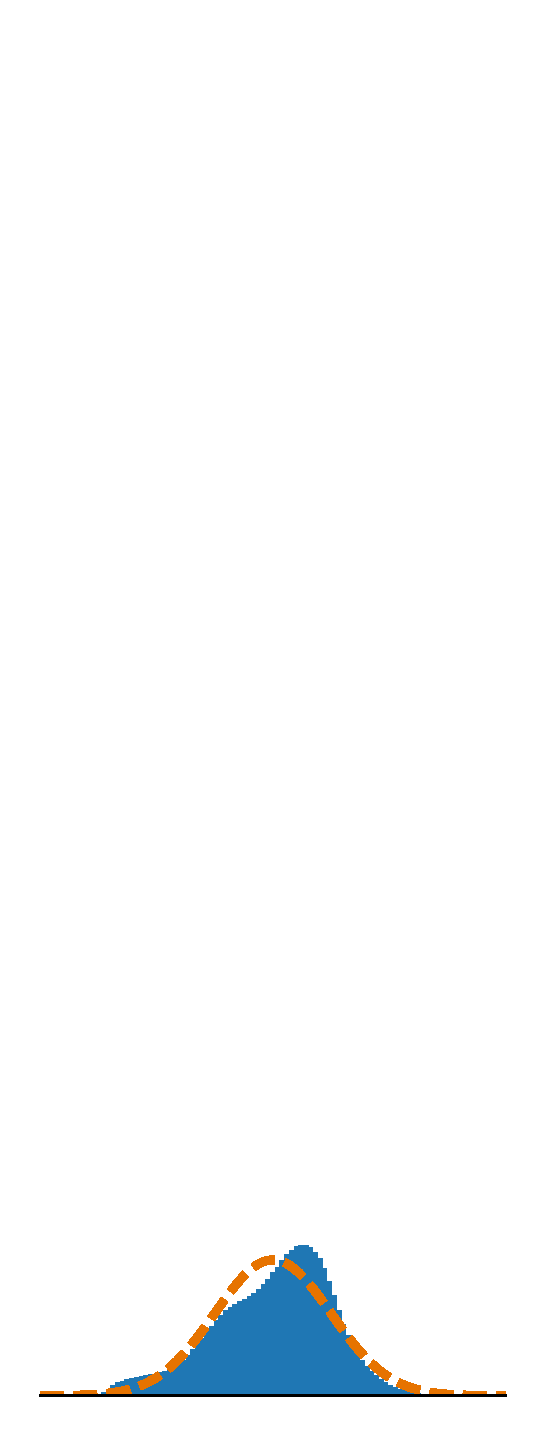
\includegraphics[width=0.33\linewidth,trim={0 0 0 20.5cm},clip]{SONYC-pcen_logE_histogram.eps}}
\stackunder{DCASE 2013 SC}{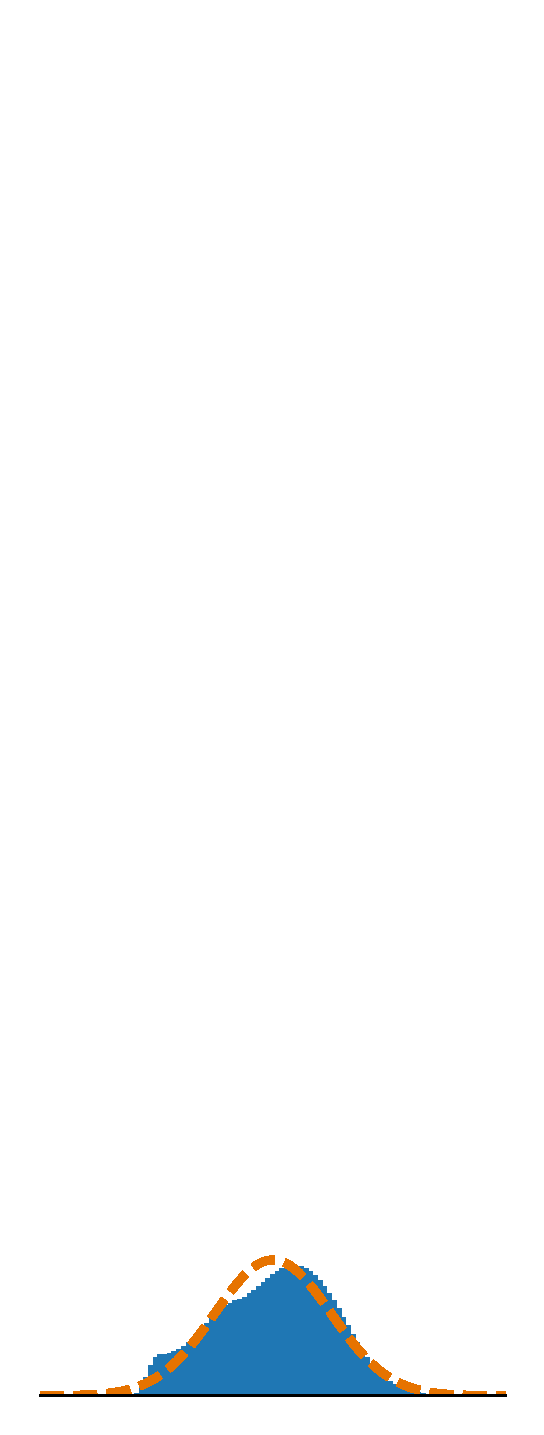
\includegraphics[width=0.33\linewidth,trim={0 0 0 20.5cm},clip]{DCASE2013-pcen_logE_histogram.eps}}
\stackunder{BirdVox}{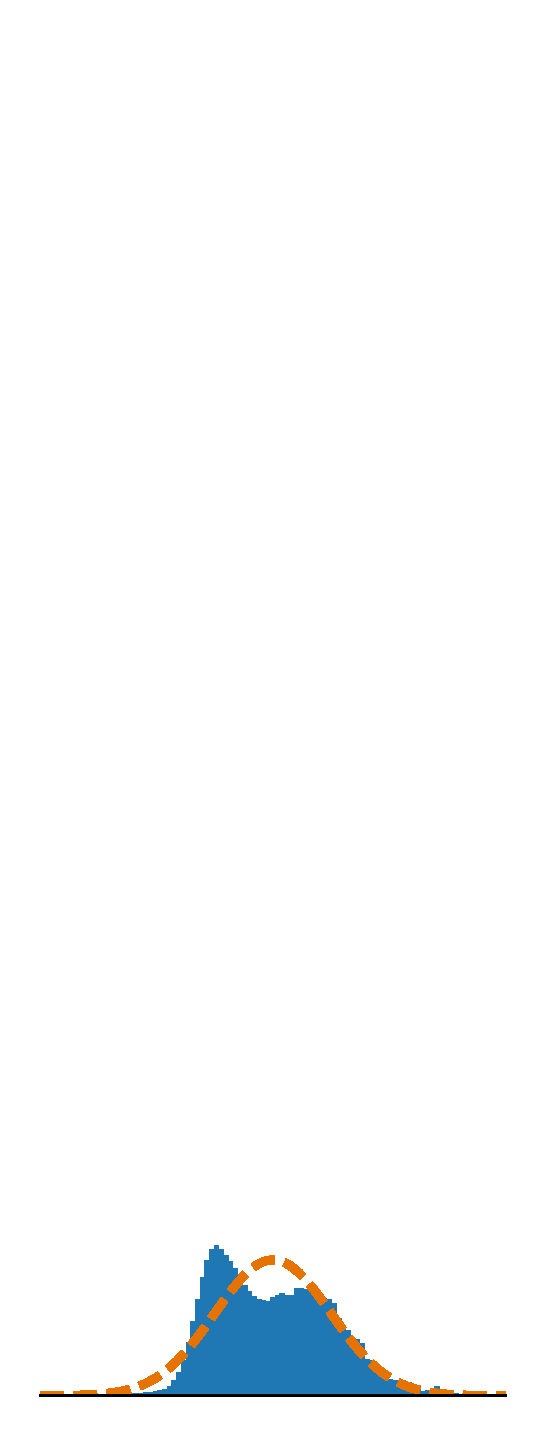
\includegraphics[width=0.33\linewidth,trim={0 0 0 20.5cm},clip]{BirdVox-pcen_logE_histogram.eps}}}
%\\
%\subfloat[Renormalization with soft threshold: $\mathbf{E} \mapsto \dfrac{\mathbf{E}}{\varepsilon+(\mathbf{E}\ast\boldsymbol{\phi})}$.]{%
%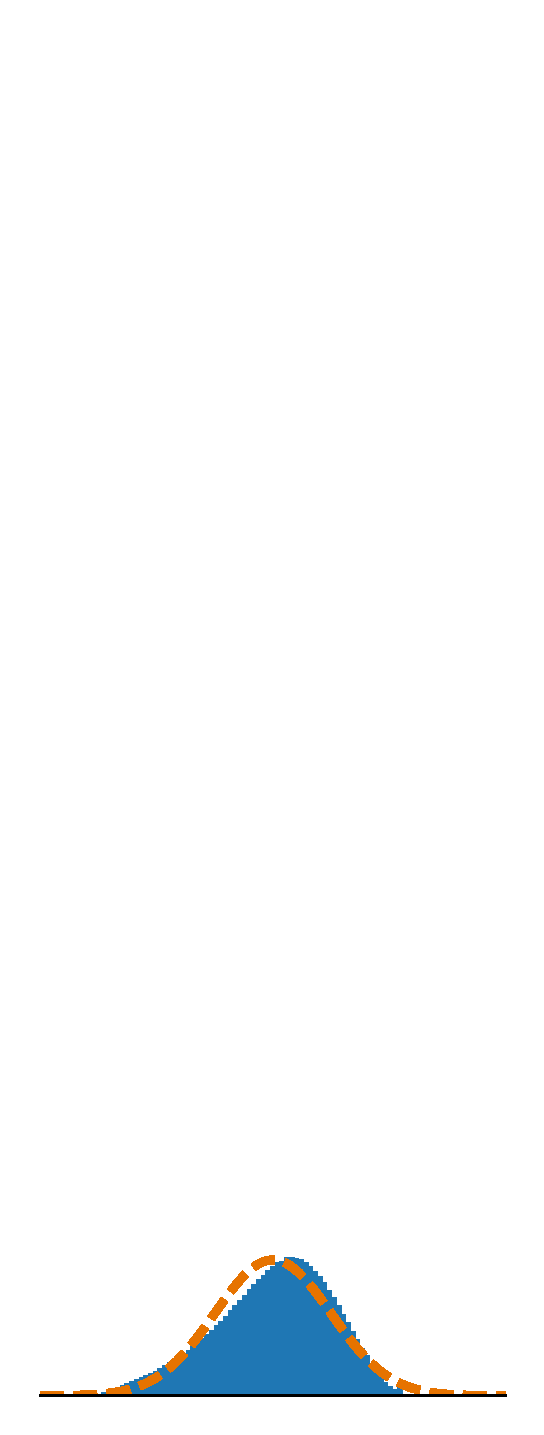
\includegraphics[width=0.33\linewidth,trim={0 0 0 20cm},clip]{SONYC-pcen_EoverMplusEps_histogram.eps}
%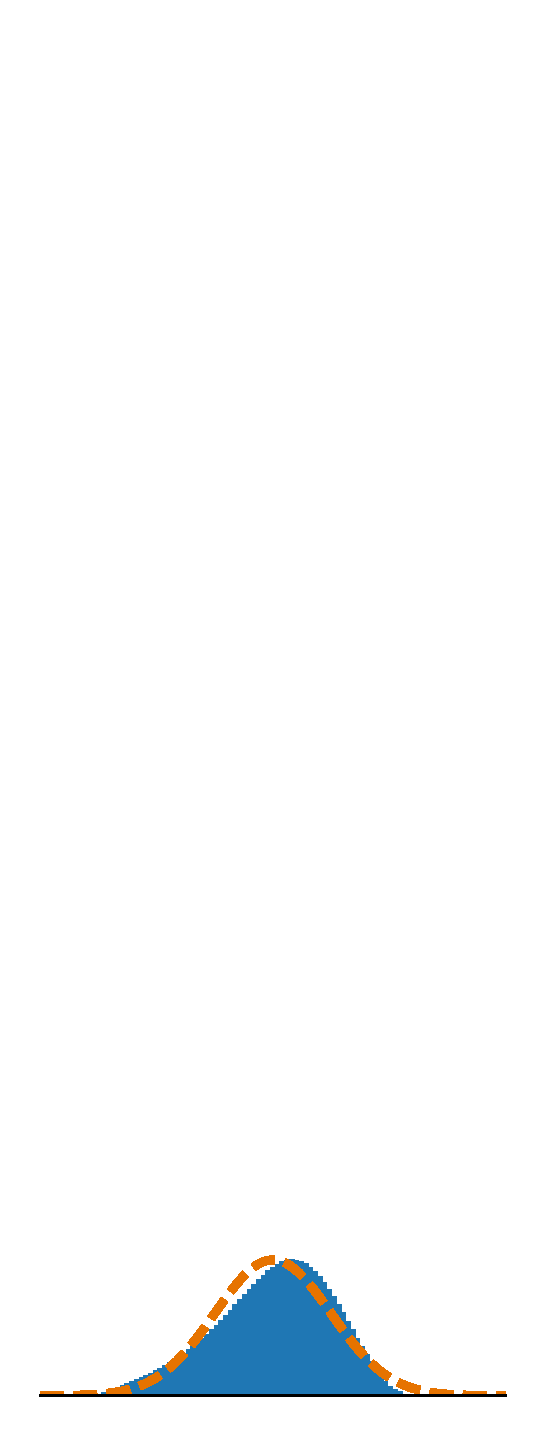
\includegraphics[width=0.33\linewidth,trim={0 0 0 20cm},clip]{DCASE2013-pcen_EoverMplusEps_histogram.eps}
%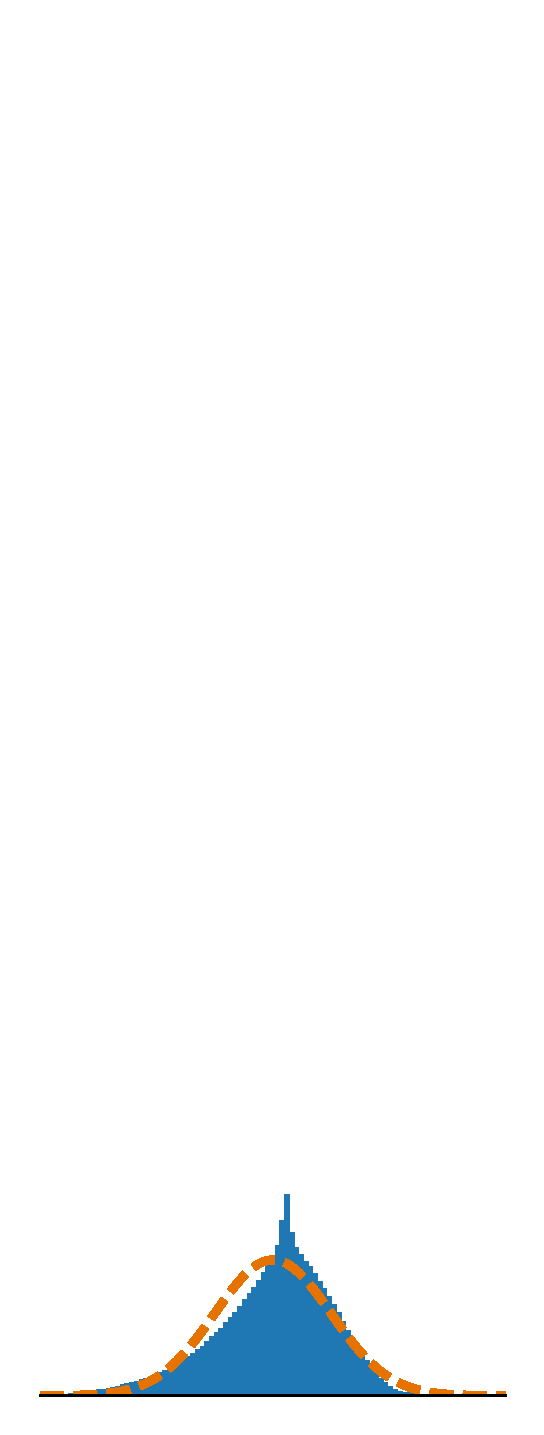
\includegraphics[width=0.33\linewidth,trim={0 0 0 20cm},clip]{BirdVox-pcen_EoverMplusEps_histogram.eps}}
%\\
%\subfloat[Renormalization with soft threshold and exponent: $\mathbf{E} \mapsto \dfrac{\mathbf{E}}{(\varepsilon+(\mathbf{E}\ast\boldsymbol{\phi}))^\alpha}$.]{%
%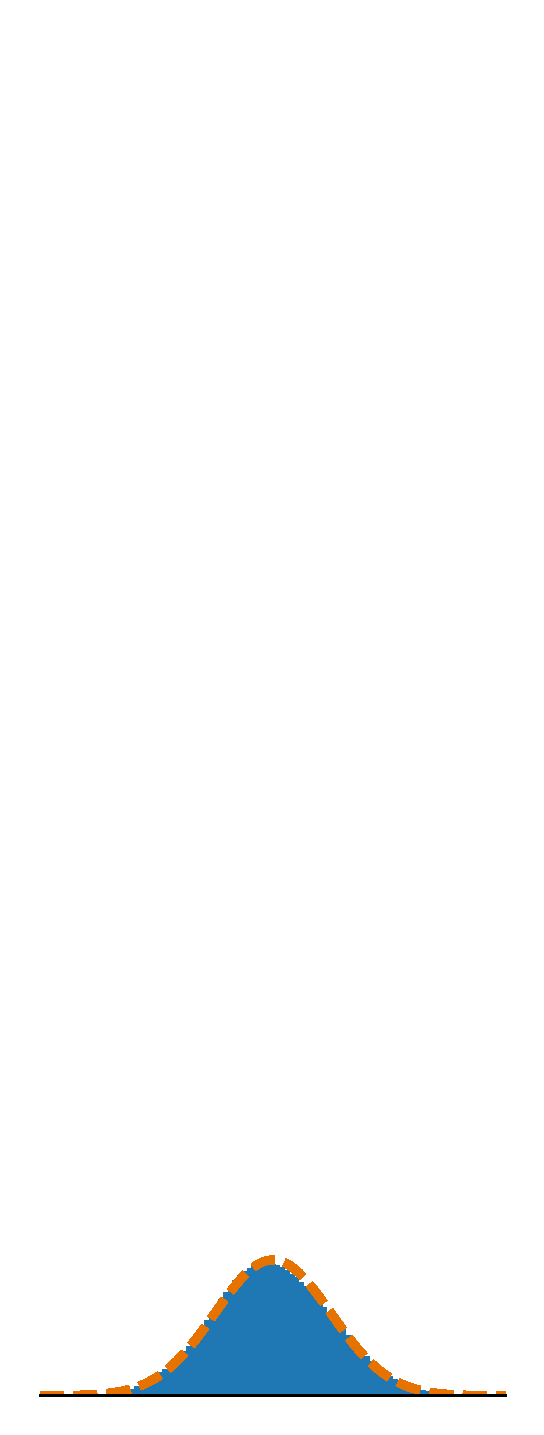
\includegraphics[width=0.33\linewidth,trim={0 0 0 20cm},clip]{SONYC-pcen_G_histogram.eps}
%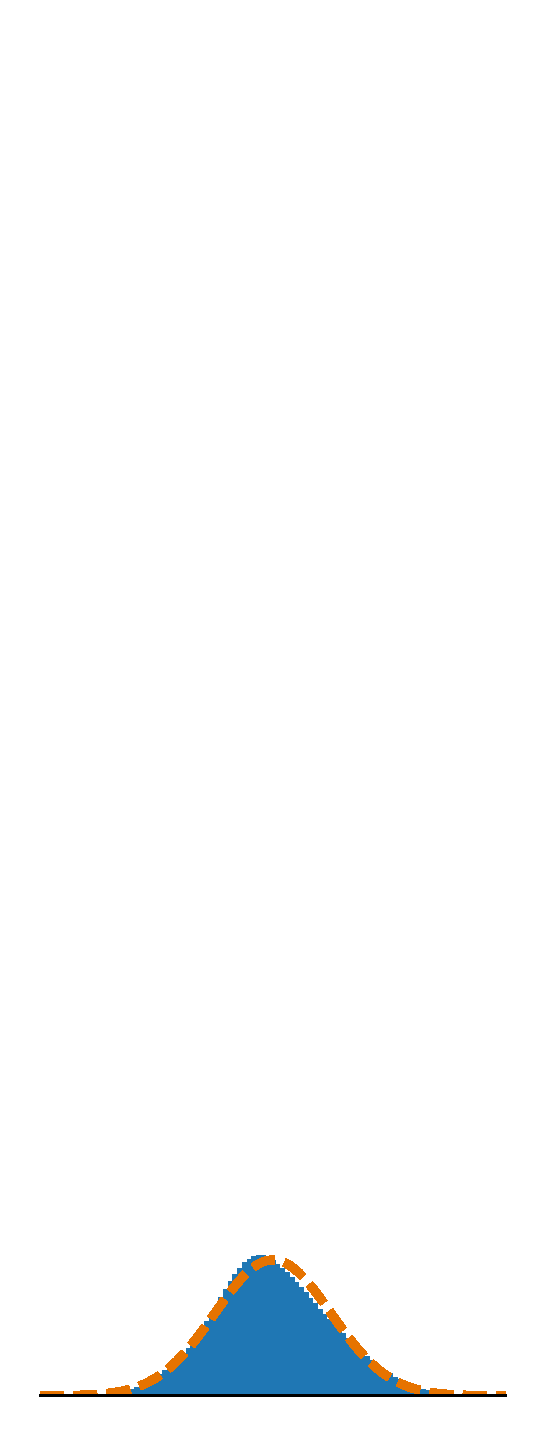
\includegraphics[width=0.33\linewidth,trim={0 0 0 20cm},clip]{DCASE2013-pcen_G_histogram.eps}
%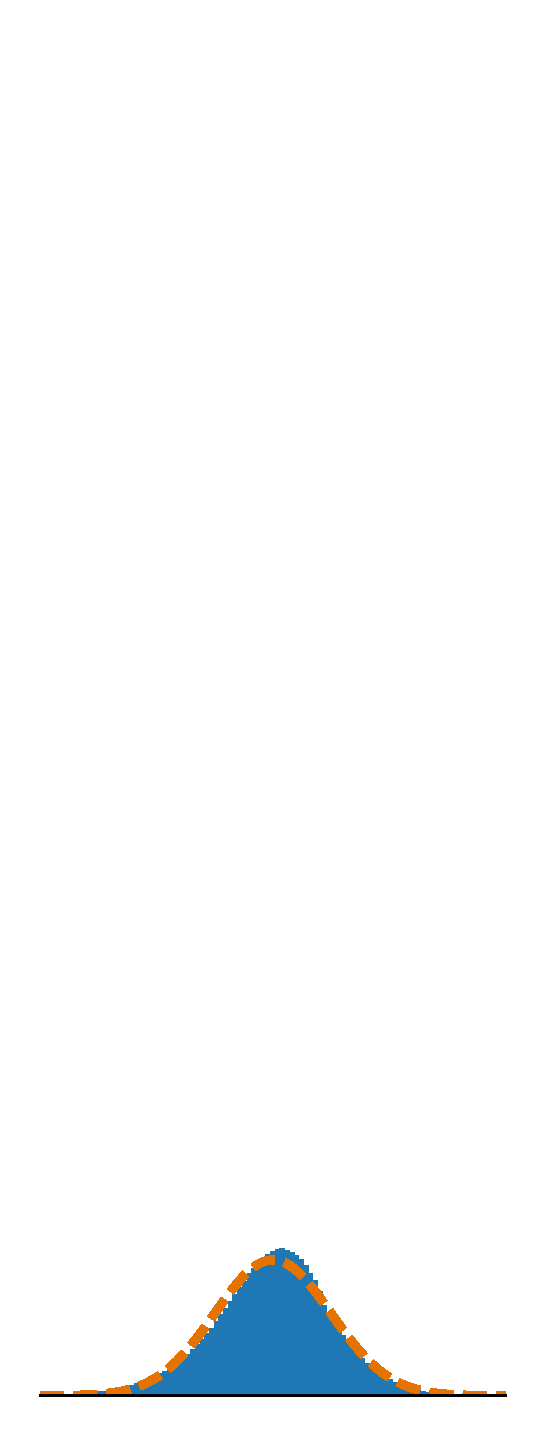
\includegraphics[width=0.33\linewidth,trim={0 0 0 20cm},clip]{BirdVox-pcen_G_histogram.eps}}
\\
\subfloat[Per-channel energy normalization (PCEN).]{%
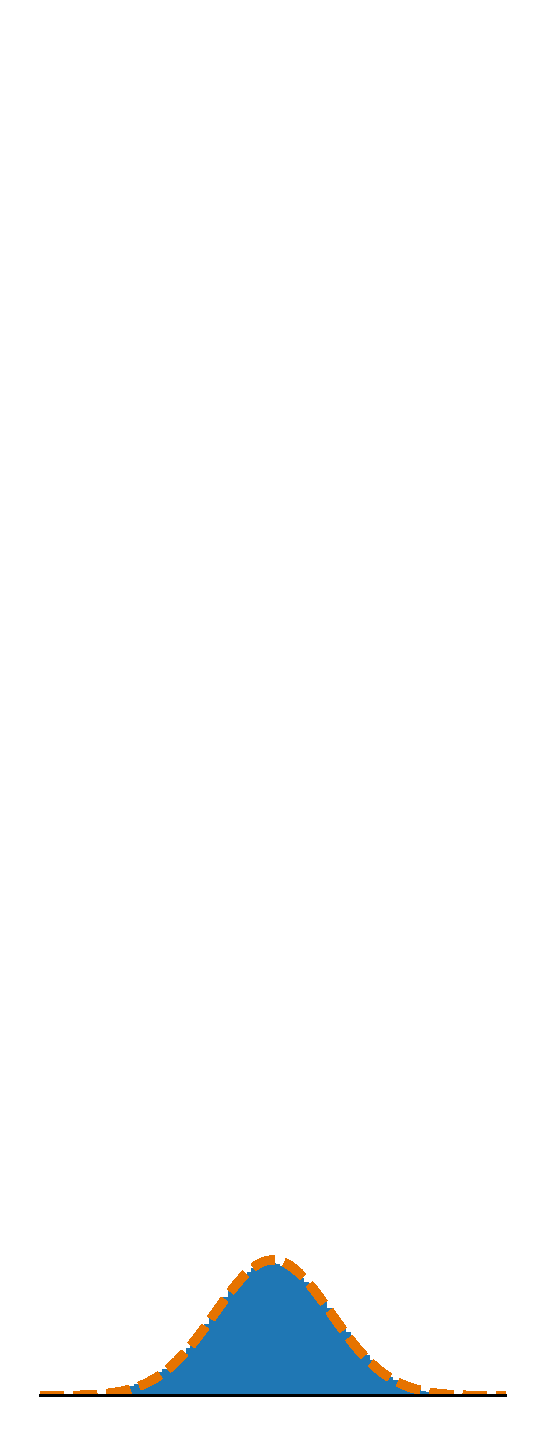
\includegraphics[width=0.33\linewidth,trim={0 0 0 21cm},clip]{SONYC-pcen_PCEN_histogram.eps}
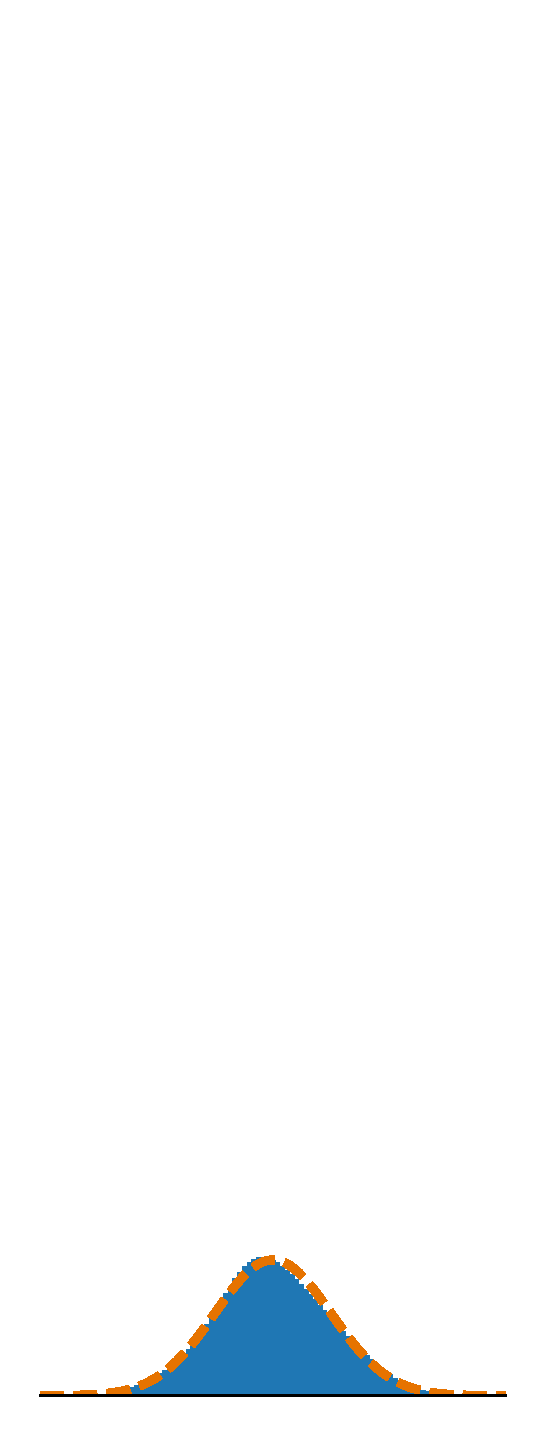
\includegraphics[width=0.33\linewidth,trim={0 0 0 21cm},clip]{DCASE2013-pcen_PCEN_histogram.eps}
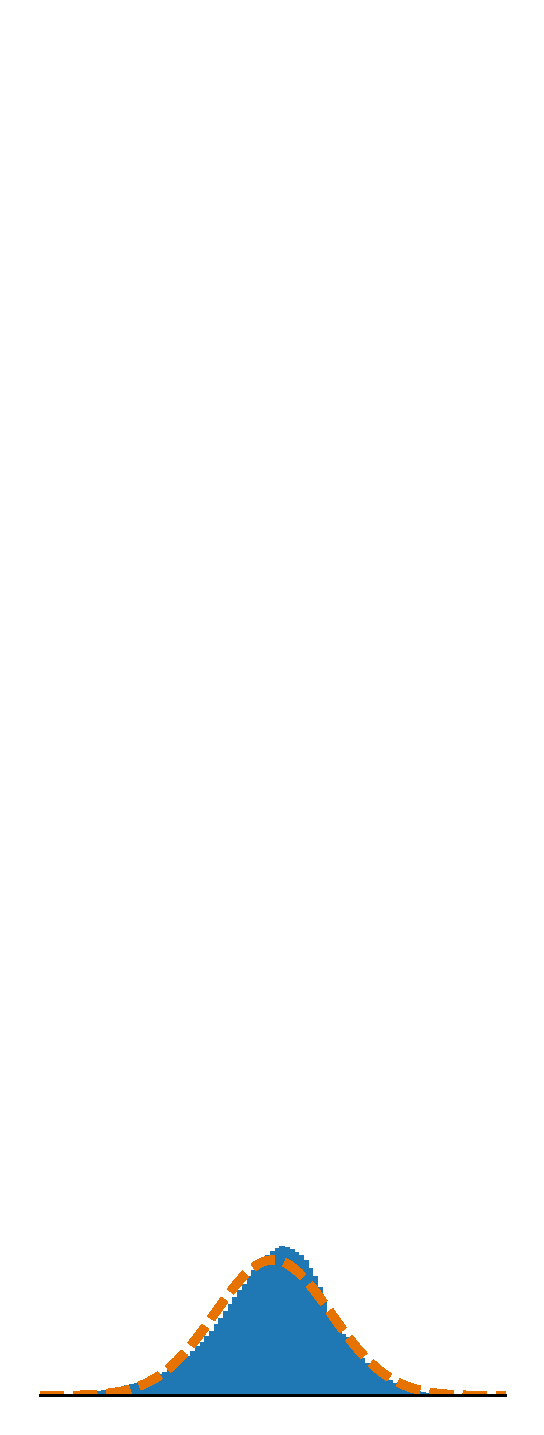
\includegraphics[width=0.33\linewidth,trim={0 0 0 21cm},clip]{BirdVox-pcen_PCEN_histogram.eps}}
\caption{Distributions of magnitudes in the mel-frequency spectrogram after logmelspec (a),  and PCEN (c), as estimated on three datasets of acoustic scenes:
SONYC (left); DCASE 2013 SC (middle); and BirdVox (right).
Each distribution is scaled to null mean and unit variance, and discretized with $500$ histogram bins ranging between $-4$ and $4$.
For comparison, the dashed line indicates the standard normal distribution.
See Subsection \ref{sub:gaussianization} for details.}
\label{fig:gaussianization}
\end{figure}

\subsection{Spectrogram whitening by decorrelation of frequency bands}\label{sub:decorrelation}
Figure \ref{fig:decorrelation} displays the covariance matrices of mel-frequency spectrogram coefficients across frequency channels.
While the logarithmic transformation suffers from strong cross-correlations between non-adjacent bands, the covariance matrix of PCEN is close to identity, thus suggesting that noise is  ``whitened''.

\begin{figure}
\centering
\subfloat[Logarithmic transformation.]{
\stackunder{SONYC}{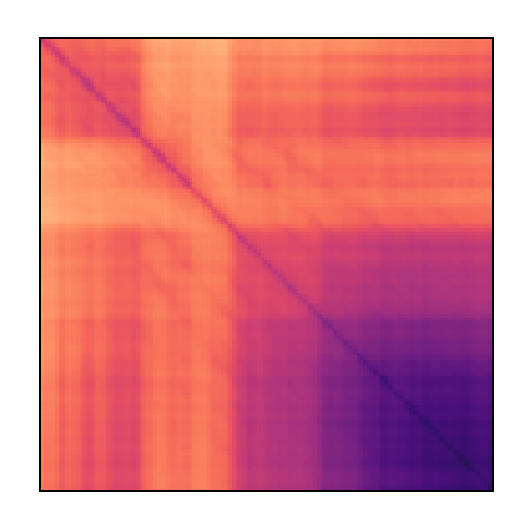
\includegraphics[width=0.33\linewidth]{SONYC-pcen_logE_covariance.eps}}
\stackunder{DCASE 2013 SC}{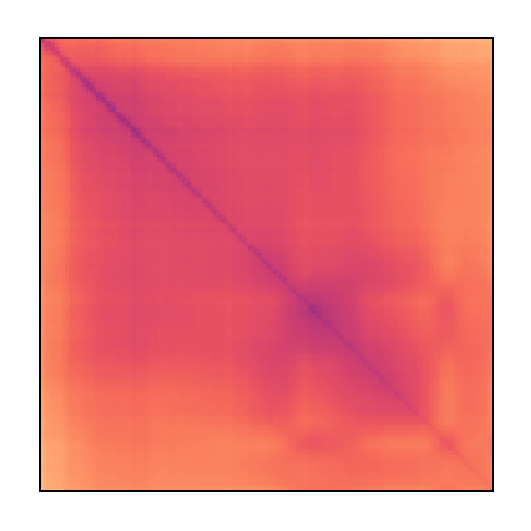
\includegraphics[width=0.33\linewidth]{DCASE2013-pcen_logE_covariance.eps}}
\stackunder{BirdVox}{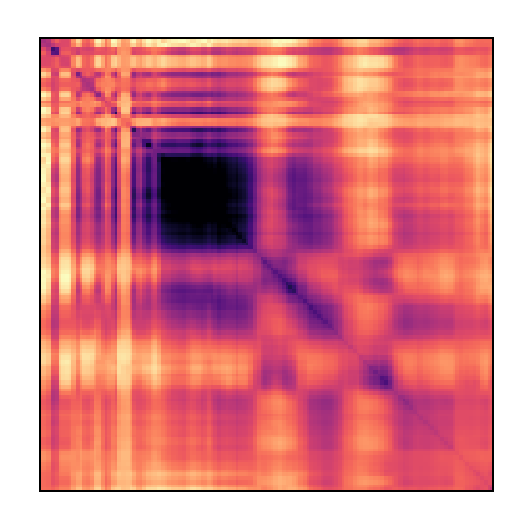
\includegraphics[width=0.33\linewidth]{BirdVox-pcen_logE_covariance.eps}}}
\\
\subfloat[Per-channel energy normalization (PCEN).]{
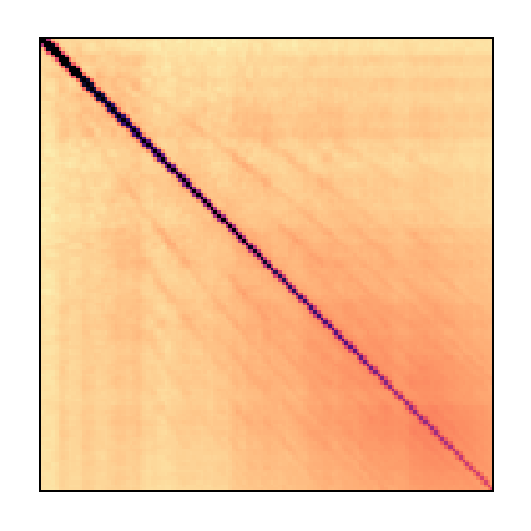
\includegraphics[width=0.33\linewidth]{SONYC-pcen_PCEN_covariance.eps}
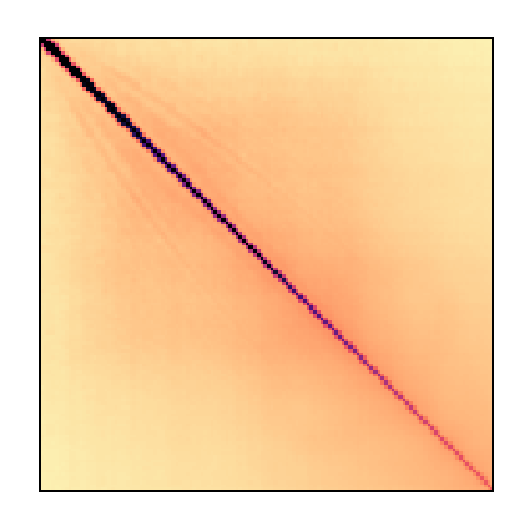
\includegraphics[width=0.33\linewidth]{DCASE2013-pcen_PCEN_covariance.eps}
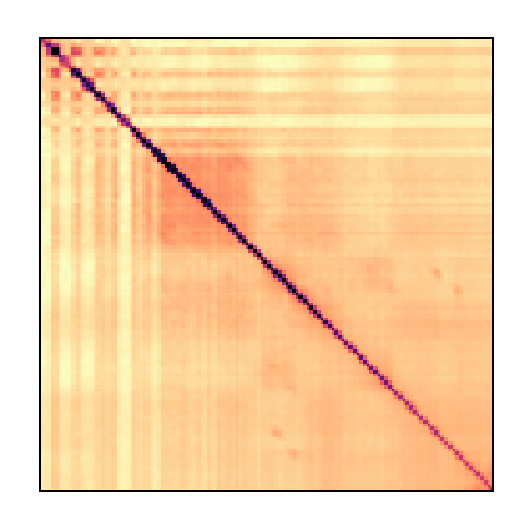
\includegraphics[width=0.33\linewidth]{BirdVox-pcen_PCEN_covariance.eps}}
\caption{Covariance matrices of frequency channels after logarithmic transformation (a) and PCEN (b), as estimated on three datasets of acoustic scenes: SONYC (left); DCASE 2013 (middle); and BirdVox (right).
Darker shades indicate larger covariances in absolute value. See Subsection \ref{sub:decorrelation} for details.}
\label{fig:decorrelation}
\end{figure}



\section{How PCEN works: an asymptotic analysis \label{sec:asymptotic}}
PCEN's ability to Gaussianize and whiten the background of acoustic recordings is the result of its three component operations of temporal integration, adaptive gain control, and dynamic range compression.
In this section, we aim to elucidate the parameter space of these three operations by means of an asymptotic analysis.
%This section decomposes PCEN into three operations: temporal integration, adaptive gain control, and dynamic range compression.
%For each of these, we derive simple asymptotic formulas from specific assumptions on $\mathbf{E}(t,f)$.
%We describe how parameters $T$, $\alpha$, $\varepsilon$, $r$, and $\delta$ affect asymptotic regimes of PCEN as well as the transitions between them.

\subsection{Temporal integration}
\label{sub:temporal-integration}
Filtering each subband $f$ in $\mathbf{E}(t,f)$ with $\boldsymbol{\phi}_T$ aims at estimating the intensity of background noise at $f$ while remaining invariant to the intensity of foreground events.
Under the assumption that the amplitude modulations (AM) of the foreground at $f$ are faster than those of the background, $T$ should be chosen to be above typical periods of foreground AM and below those of background AM.
The same can be said of frequency modulation (FM): PCEN enhances chirped events in the mel-frequency spectrogram that move from one subband $f$ to the next in less time than $T$ while attenuating slower FM.
Thus, $T$ is the transition threshold between a stationary regime of background and a transient regime of foreground.

The original implementation of PCEN \cite{wang2017icassp} defines $\boldsymbol{\phi}_T (t)$ as a first-order IIR filter whose response to $\mathbf{E}(t,f)$ is
\begin{equation}
\mathbf{M}(t,f) = (\mathbf{E} \ast \boldsymbol{\phi}_T)(t,f) = s \mathbf{E}(t,f) + (1-s) \mathbf{M}(t - \tau,f),
\label{eq:autoregressive}
\end{equation}
where $0<s<1$ is the weight of the associated autoregressive process ($\mathrm{AR}(1)$) and $\tau$ is the discretization time step (``hop size'') in seconds.

\begin{prop}
The autoregressive filter $\boldsymbol{\phi}_T$ defined in Equation \ref{eq:autoregressive} is a low-pass filter of gain $\SI{0}{\decibel}$, cutoff frequency
$\omega_\mathrm{c} = \frac{2\pi\tau}{T} = \arccos(1 - \frac{s^2}{2 (1-s)})$ at \SI{3}{\decibel}, and sidelobe falloff of \SI{10}{\decibel} per decade near $\omega_\mathrm{c}$.
\label{prop:temporal-integration}
\end{prop}

Figure \ref{fig:temporal-integration} illustrates the frequency response of $\boldsymbol{\phi}_T$ for different values of $T$.

\begin{figure}
\centering
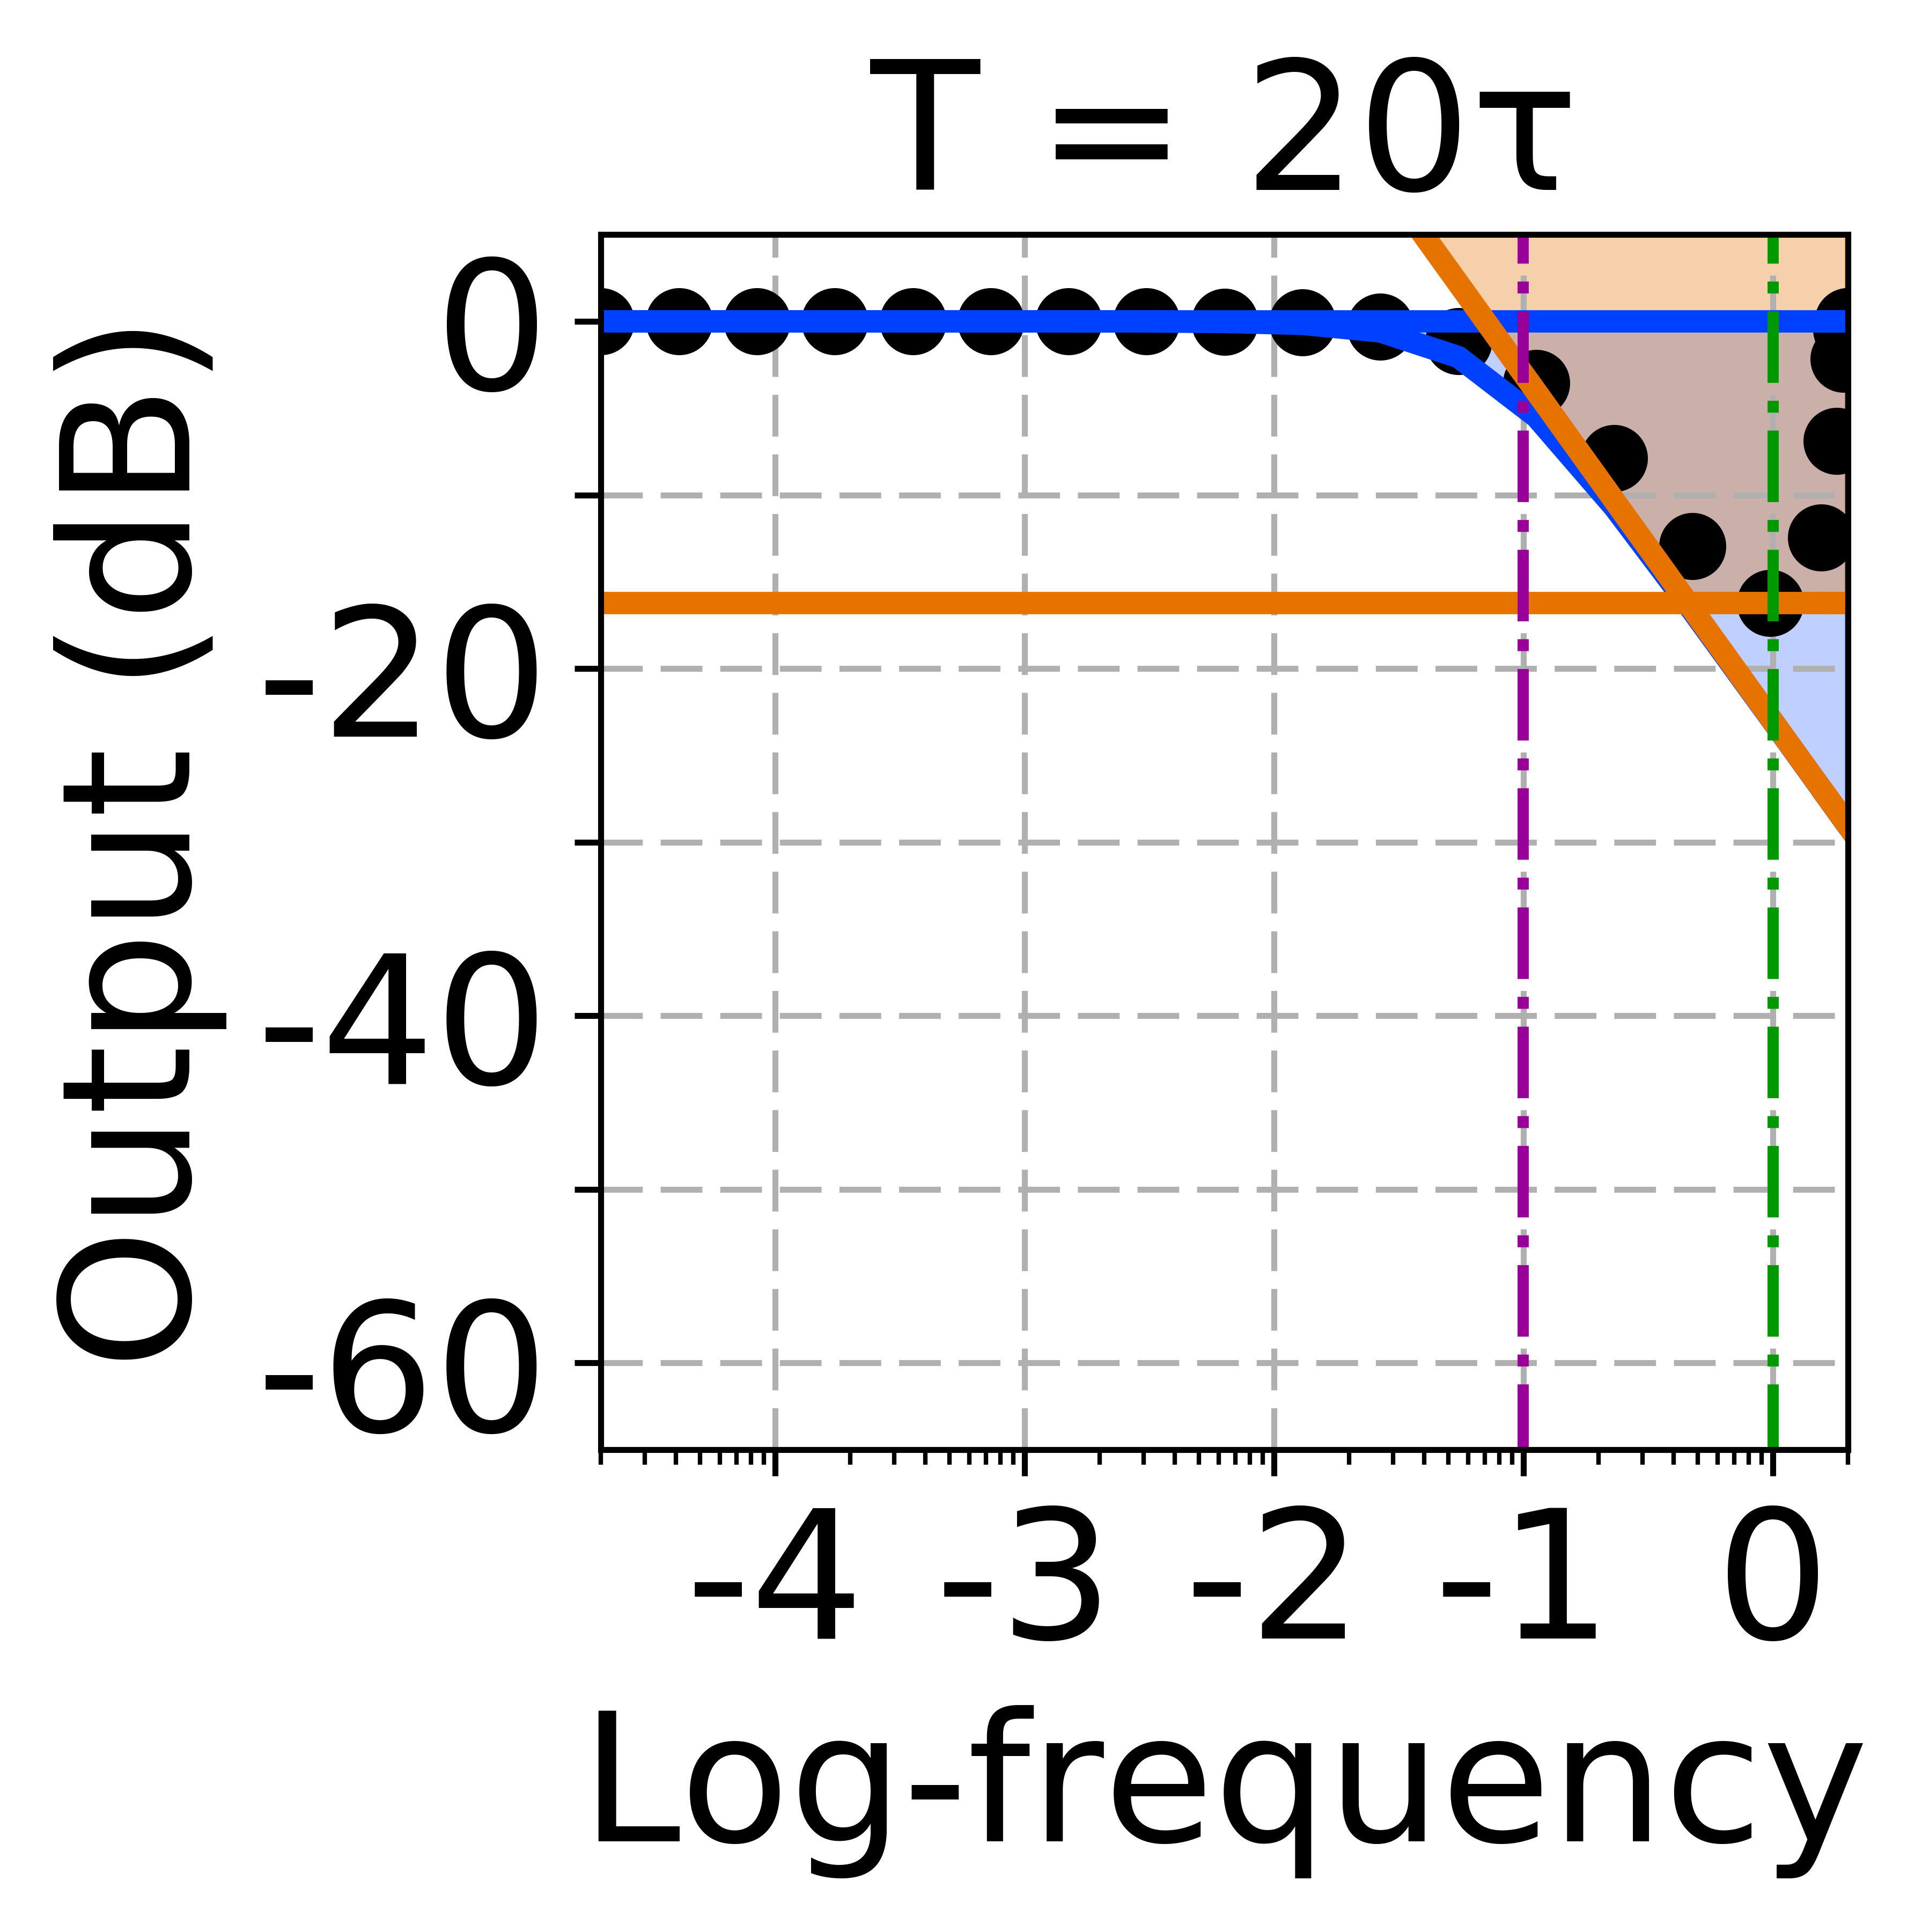
\includegraphics[height=0.33\linewidth]{frequency_response_T_20.png}
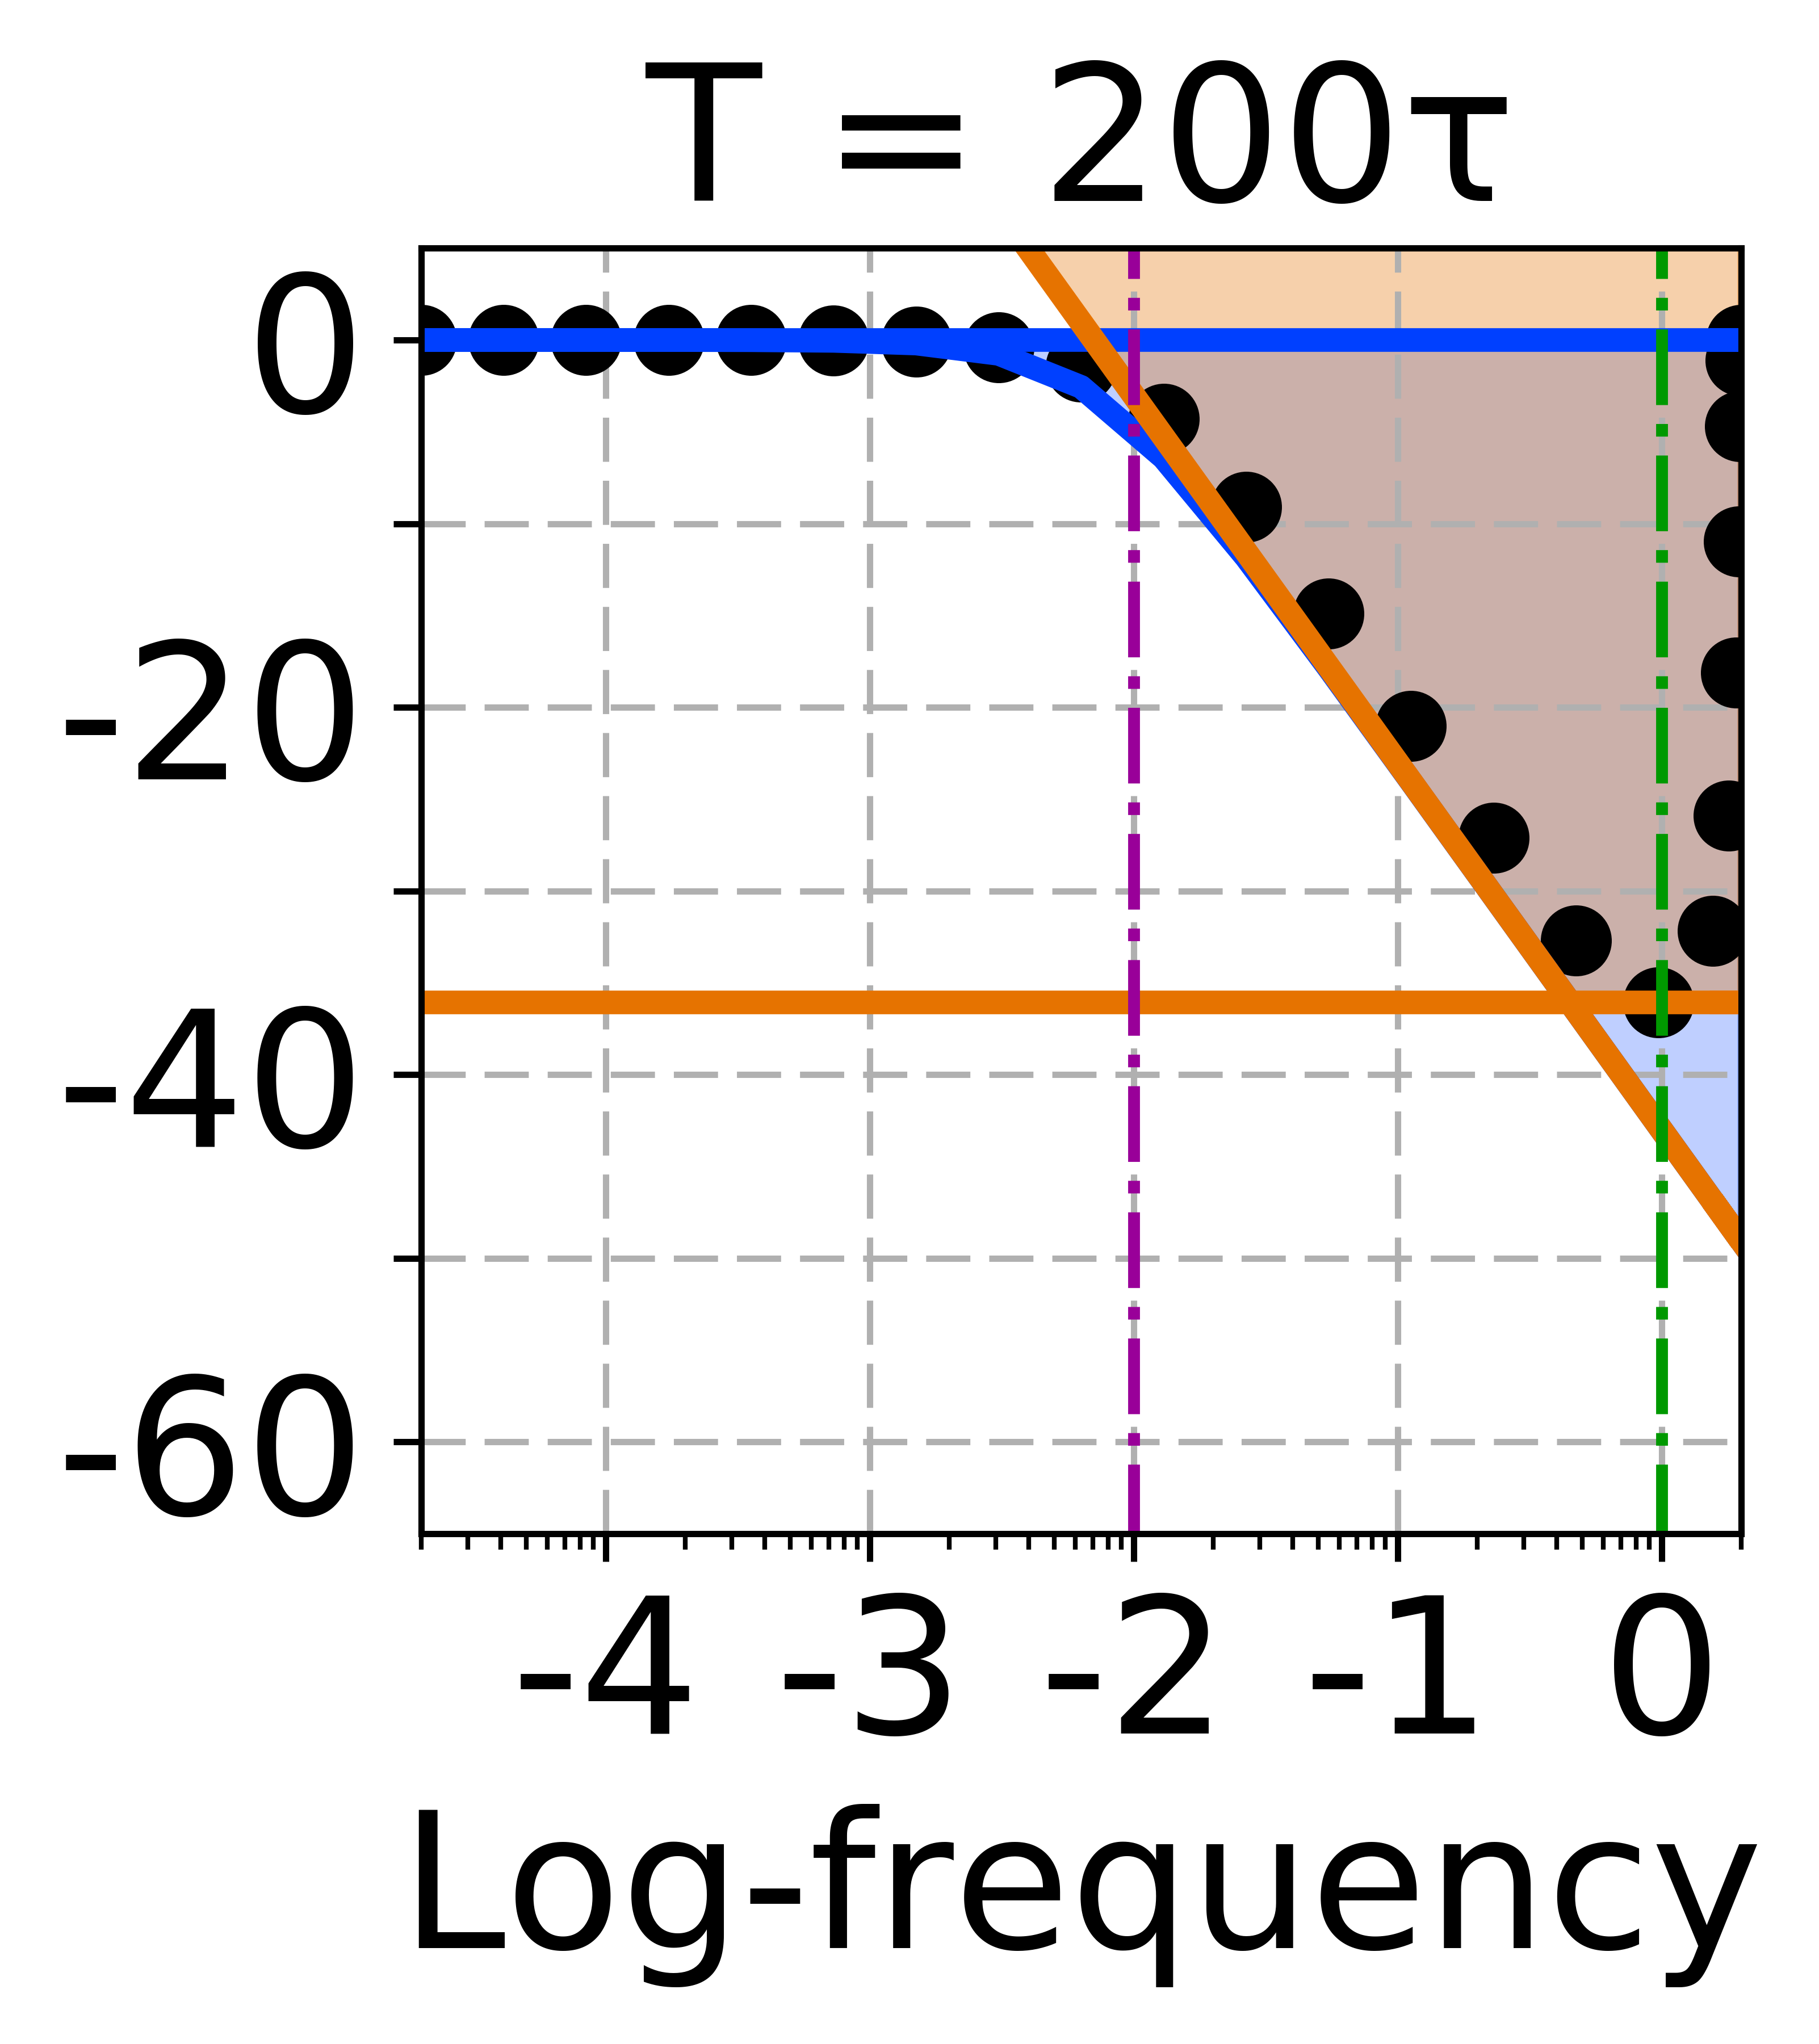
\includegraphics[height=0.33\linewidth]{frequency_response_T_200.png}
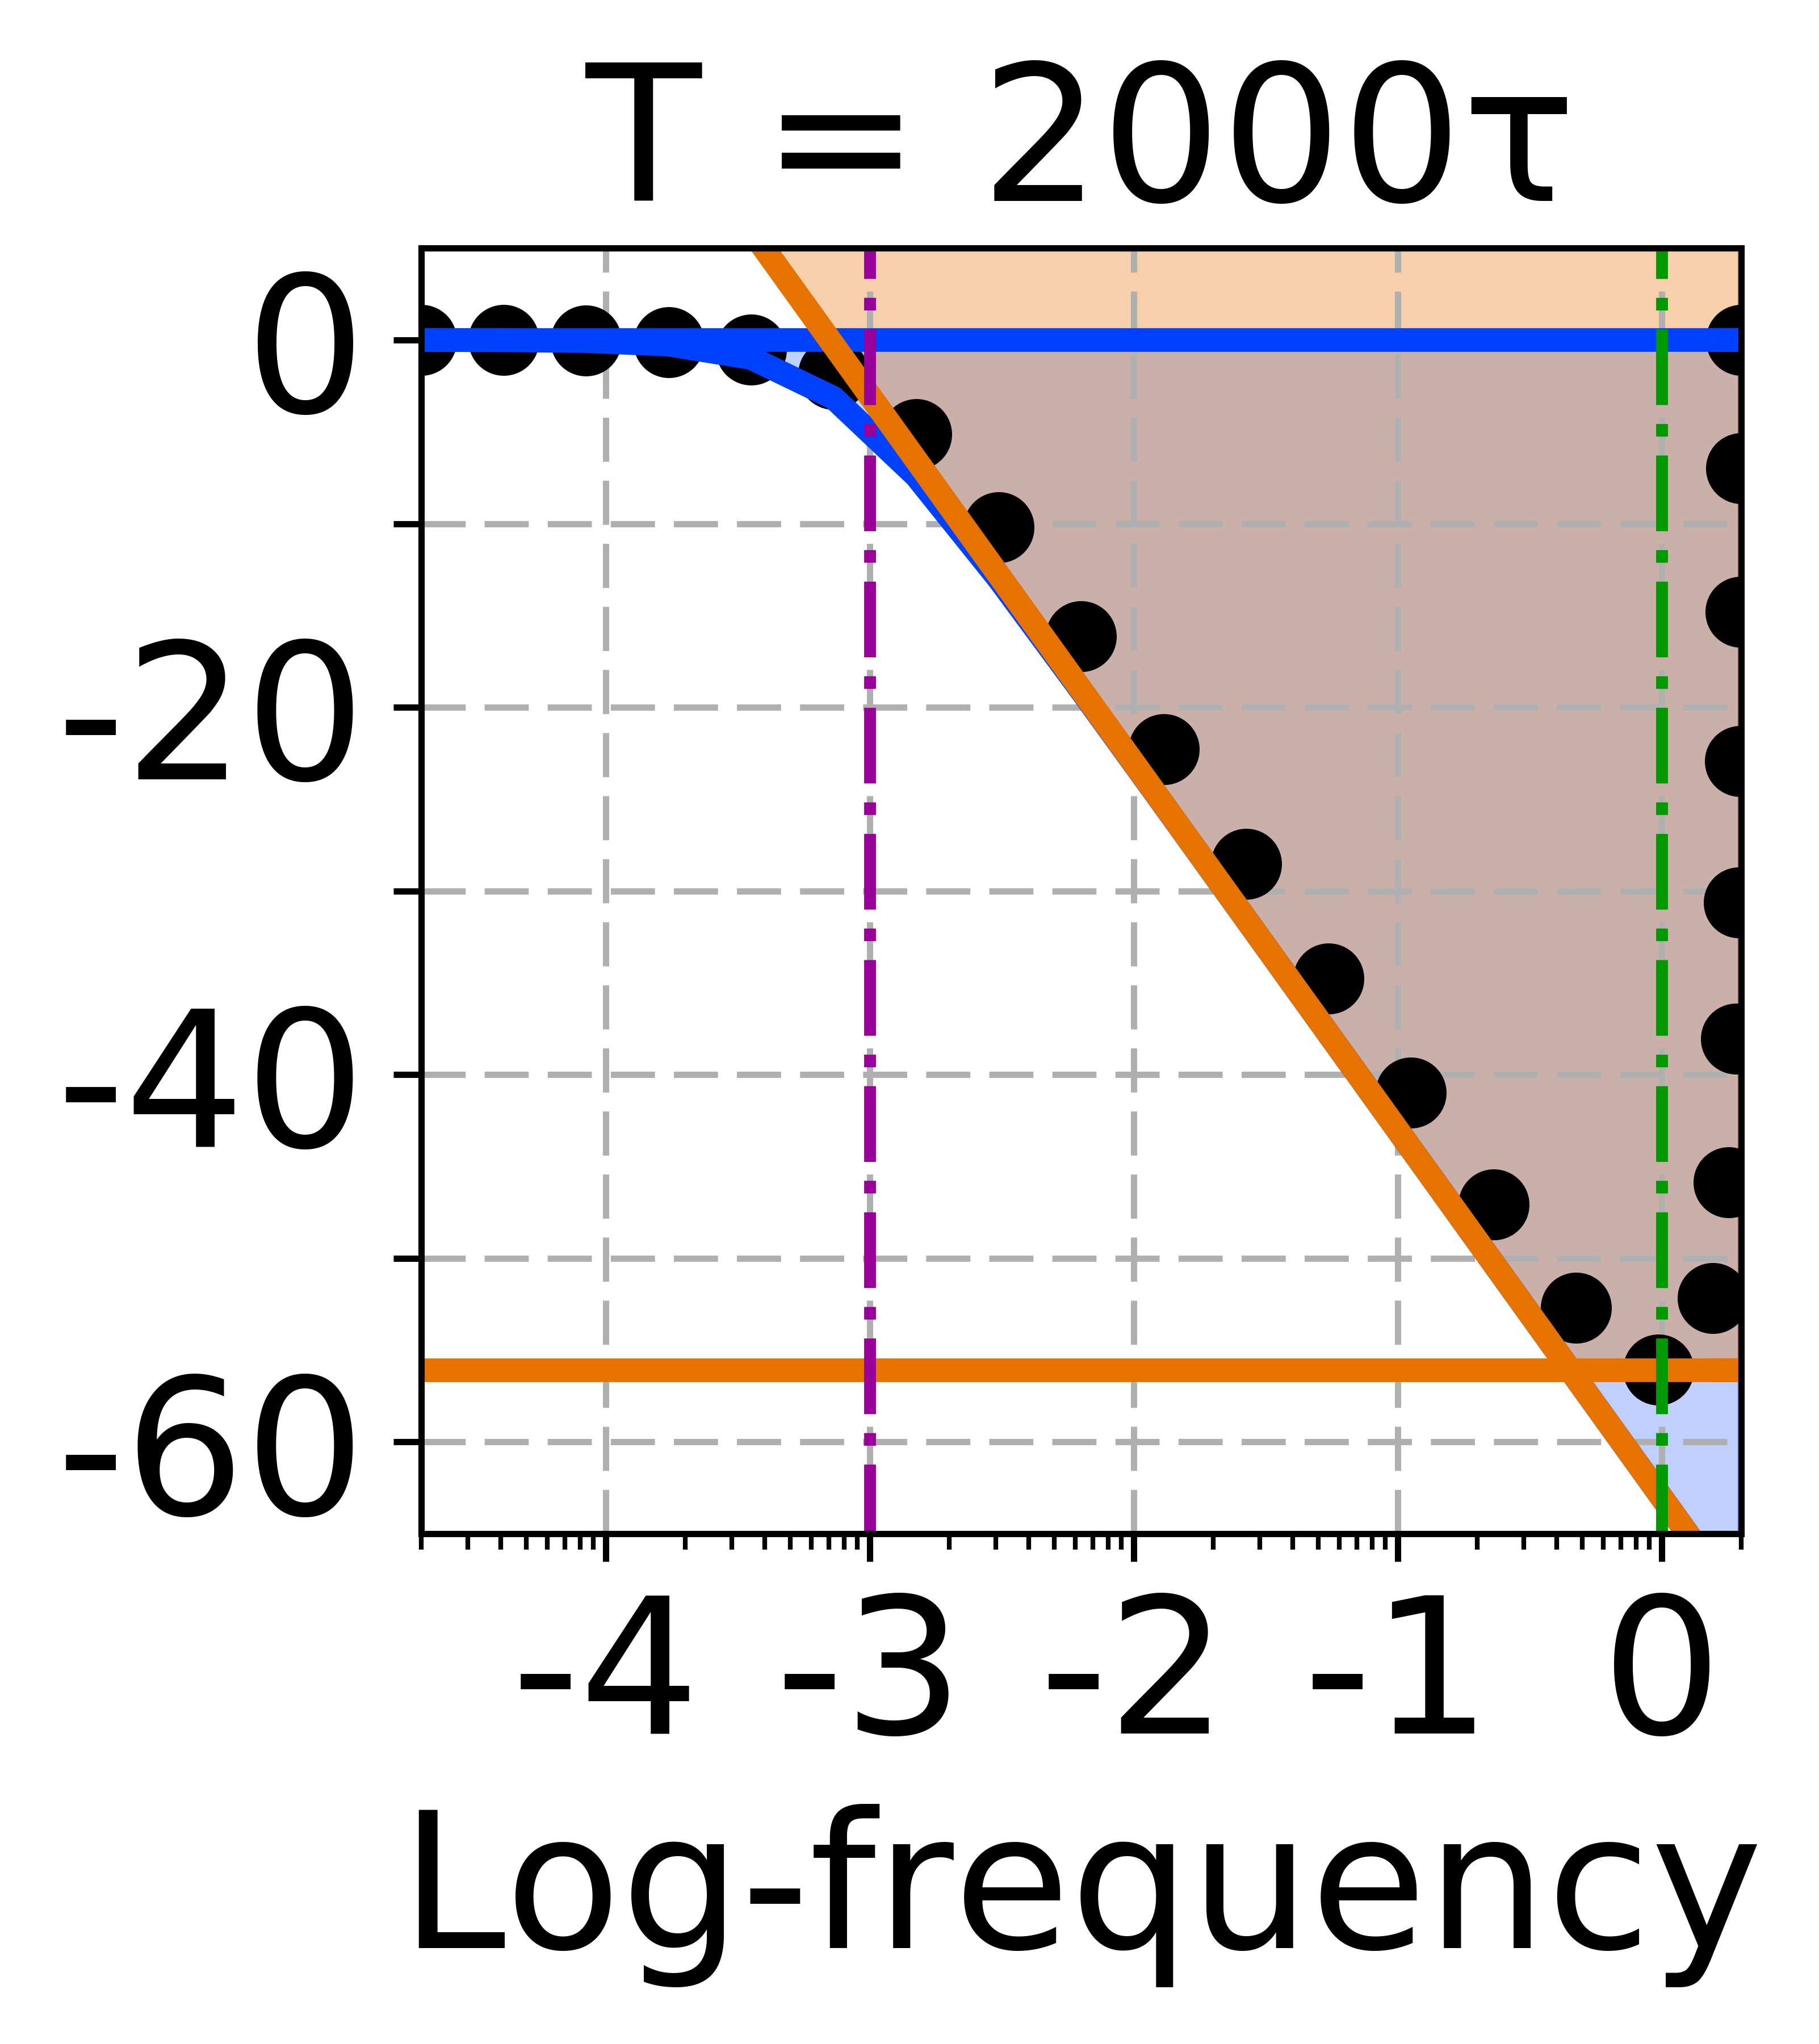
\includegraphics[height=0.33\linewidth]{frequency_response_T_2000.png}

\includegraphics[height=0.5cm]
{frequency_response_legend.png}
\caption{Bode plot of the filter $\vert \widehat{\boldsymbol{\phi}_T}(\omega) \vert^2$, measured in relative magnitude (dB) as a function of the ratio $\frac{\omega}{\omega_\mathrm{c}}$ between frequency and cutoff frequency $\omega_\mathrm{c} = \frac{2\pi\tau}{T}$.
The time scale $T$ is alternatively set to $10^{1} 2\tau$ (left), $10^{2} 2\tau$ (middle), and $10^{3} 2\tau$ (right).
We observe
%a gain of $\SI{0}{\decibel}$ in the passband and
a sidelobe falloff of \SI{10}{\decibel} per decade in the stopband.
Solid lines and shaded areas respectively denote asymptotic bounds and their corresponding error margins, as proved in Proposition \ref{prop:temporal-integration}.
The dashed purple (\resp{} green) vertical line denotes the cutoff (\resp{} Nyquist) frequency.
\label{fig:temporal-integration}}
\end{figure}

\subsection{Adaptive gain control (AGC)}
The smoothed mel-frequency spectrogram $\mathbf{M}(t,f)$ estimates the level of stationary background noise level in each frequency band $f$ (where background is defined as slower AM than $T$), and serves to adapt the gain level in the denominator of the following equation:
\begin{equation}
\mathbf{G}(t,f) = \dfrac{ \mathbf{E}(t,f) }{ (\mathbf{M}(t,f)+\varepsilon)^\alpha},
\label{eq:gain-control}
\end{equation}
where $0 < \alpha < 1$ (\resp{} $\varepsilon > 0$) is the exponent (\resp{} soft threshold) of AGC.
This stage resembles mean-variance renormalization \cite{chen2007taslp}, relative spectra (RASTA) \cite{hermansky1994tsap}, and cepstral mean normalization \cite{atal1974jasa}. 

The parameter $\varepsilon$ distinguishes two regimes: silent ($\mathbf{M}(t,f) \ll \varepsilon$) and active ($\mathbf{M}(t,f) \gg \varepsilon$).
Multiplying $\mathbf{E}(t,f)$ by some constant $C$ leads to $\mathbf{G}(t,f)$ being multiplied by approximately $C$ in the silent regime and by $C^{1-\alpha}$ in the active regime.
For $\varepsilon$ of the order of unit roundoff and $\alpha$ close to $1$, the following proposition proves that AGC is nonexpansive in quasi-silent frequency bands and strongly compressive in active frequency bands.

\begin{prop}
$\mathbf{G}(t,f)$ is asymptotically equivalent to: (i) $\mathbf{E}(t,f) / \varepsilon^\alpha$ if $\mathbf{M}(t,f) \ll \varepsilon$ and to (ii) $\mathbf{E}(t,f) / \mathbf{M}(t,f)^\alpha$ if $\mathbf{M}(t,f) \gg \varepsilon$.
\label{prop:gain-control}
\end{prop}

Figure \ref{fig:gain-control} illustrates the empirical fit of the characteristic $\mathbf{M} \mapsto (\mathbf{M}+\varepsilon)^{-\alpha}$ to the asymptotic regimes described in Proposition \ref{prop:gain-control}.
In the active regime, bringing $\alpha$ closer to $1$ (\resp{} to $0$) leads to more (\resp{} less) cancellation of background noise.

In the limit case $\varepsilon = 0$ and $\alpha = 1$, the proposition below proves that spectral equalization does not affect $\mathbf{G}$, because its effect on the numerator $\mathbf{E}$ is compensated by AGC with $\mathbf{M}$.

\begin{prop}\label{prop:invariance}
Let $\mathbf{h}(t)$ be the impulse response of some acoustic environment or recording device. If $\vert\widehat{\mathbf{h}}\vert(f) = 0$ for $f < \frac{1}{T}$ and $\vert\widehat{\mathbf{h}}\vert(f) > 0$ for every $f$ in the audible range, $\mathbf{G}$ is invariant to the filtering of the underlying waveform by $\mathbf{h}$.
\end{prop}

This result, derived from \cite{anden2014taslp}, makes PCEN suitable for remote sensing applications, where acoustic models need to be robust to variations in the absorption properties of the environment, as well as in sensor technology \cite{katsamanis2014icassp,lostanlen2017phd}.

\begin{figure}
\centering
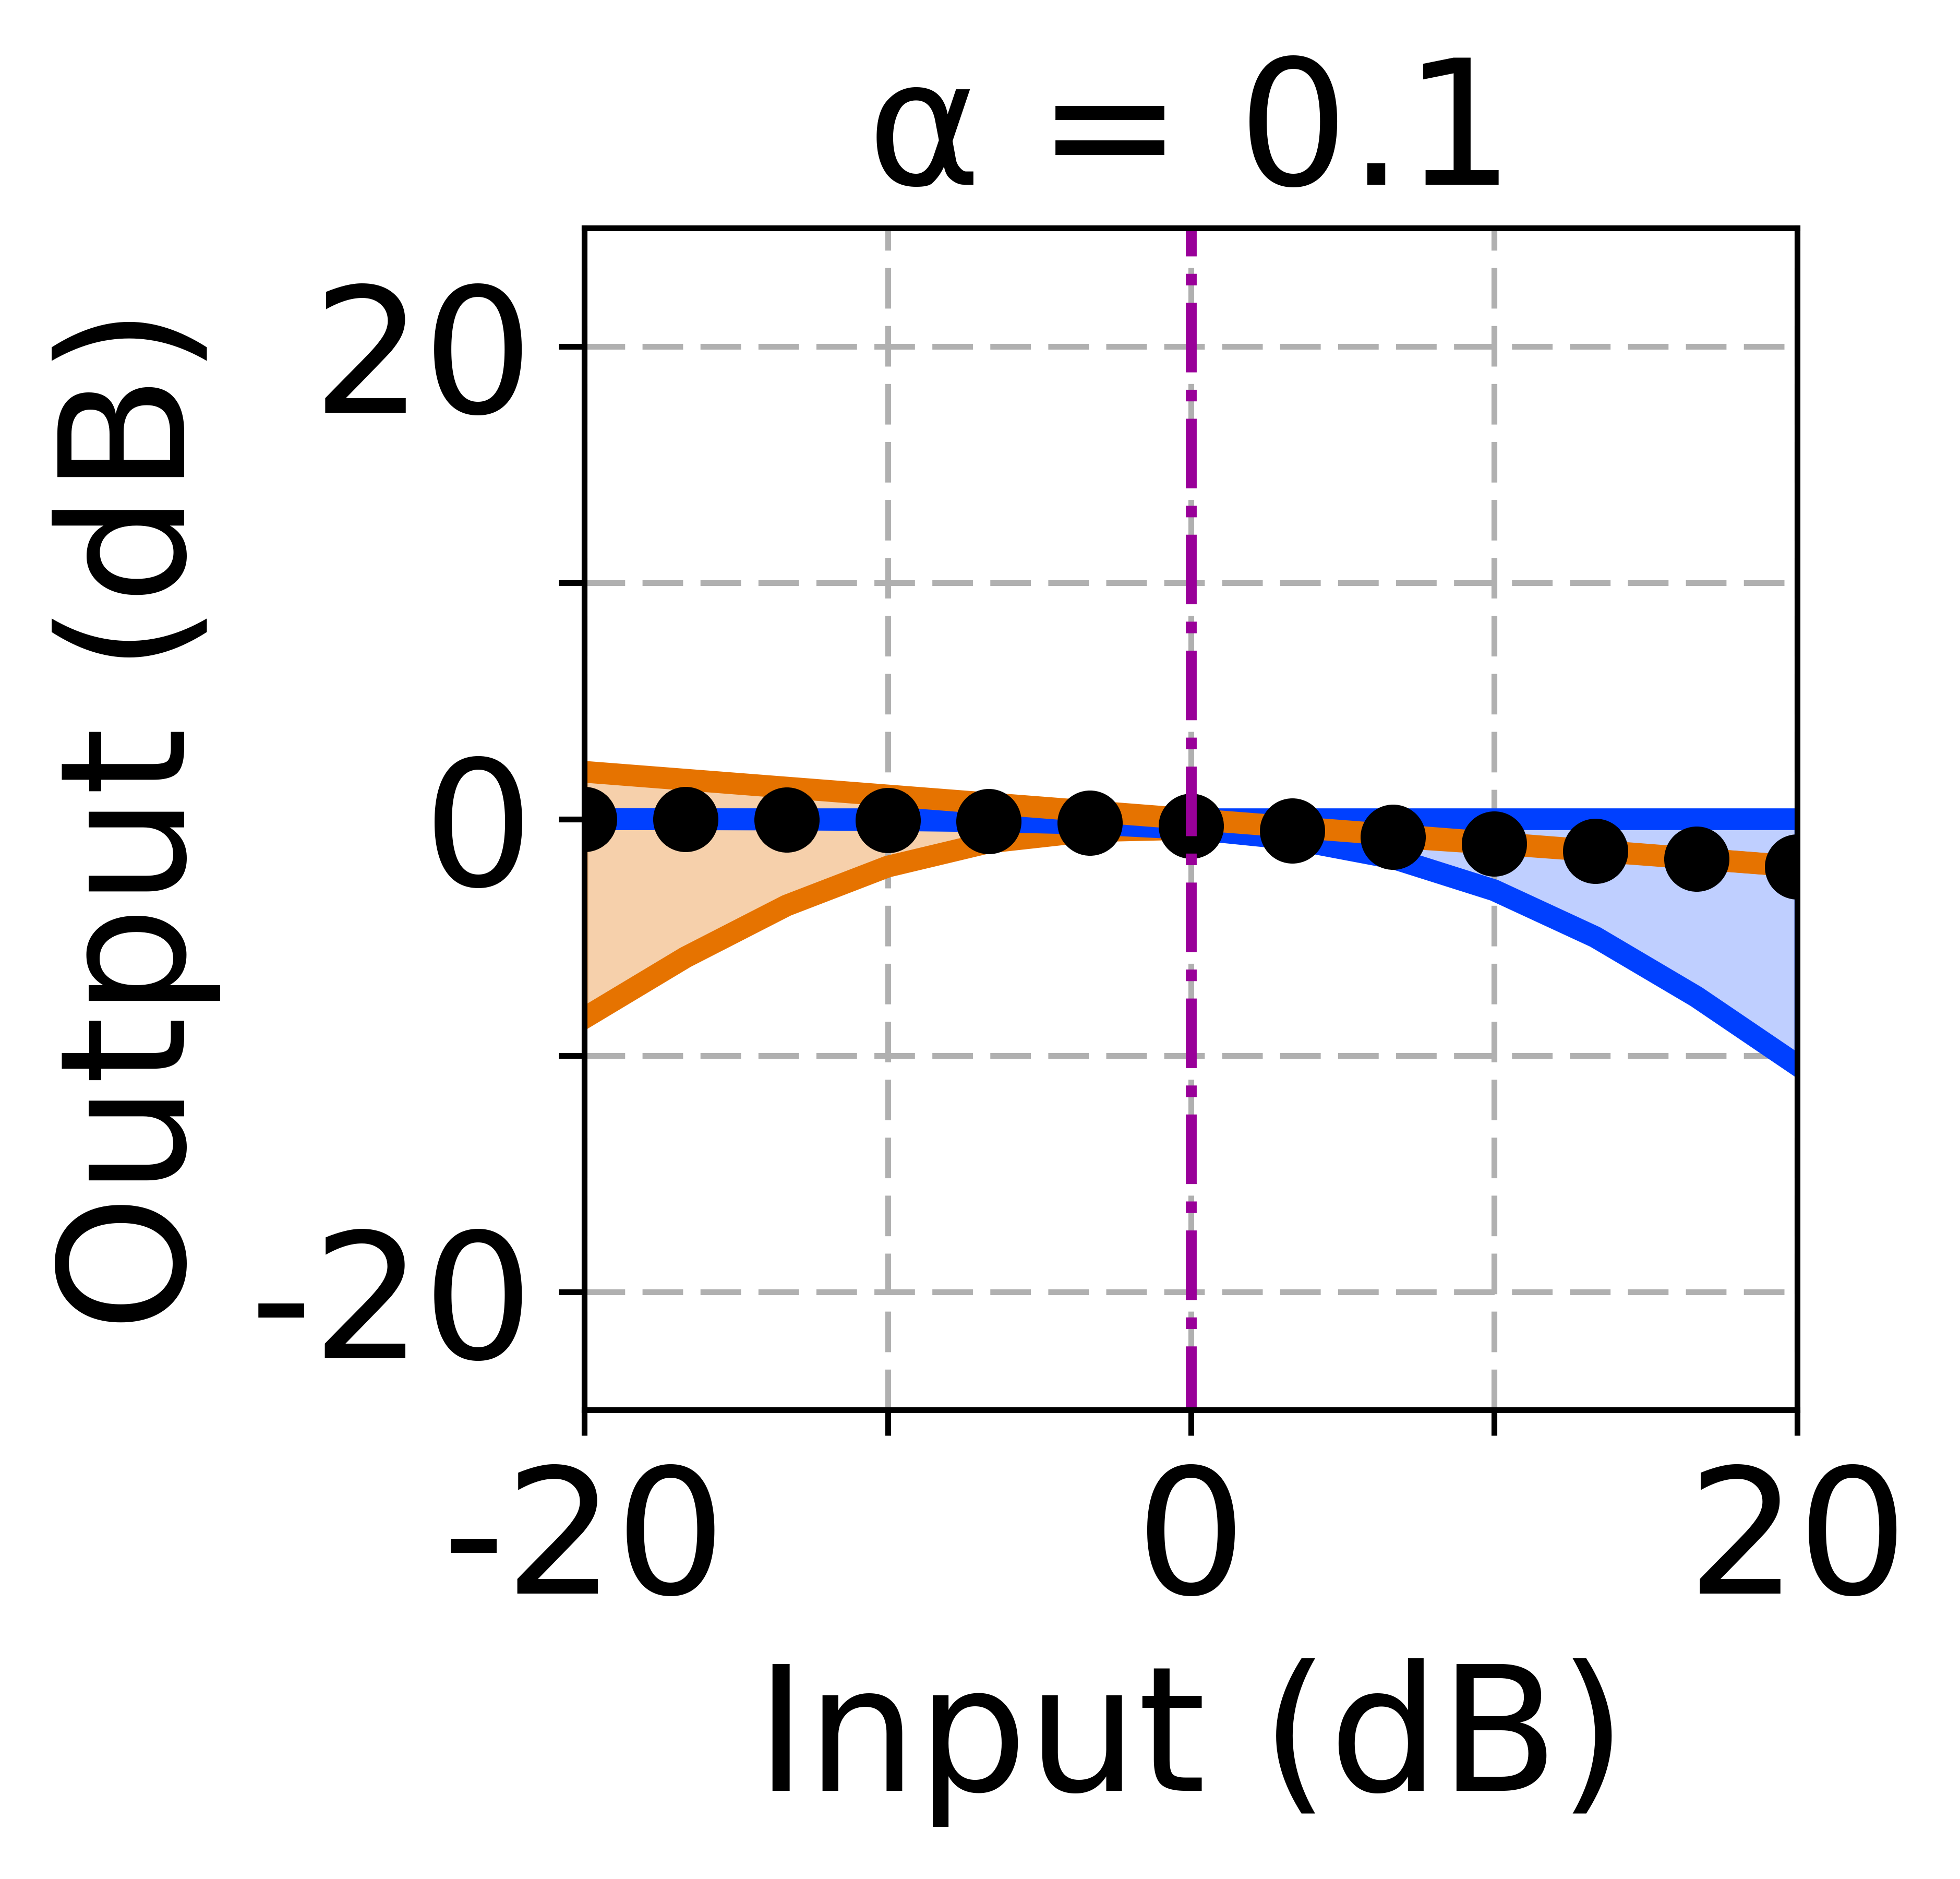
\includegraphics[height=0.33\linewidth]
{bode_renorm_0_1.png}
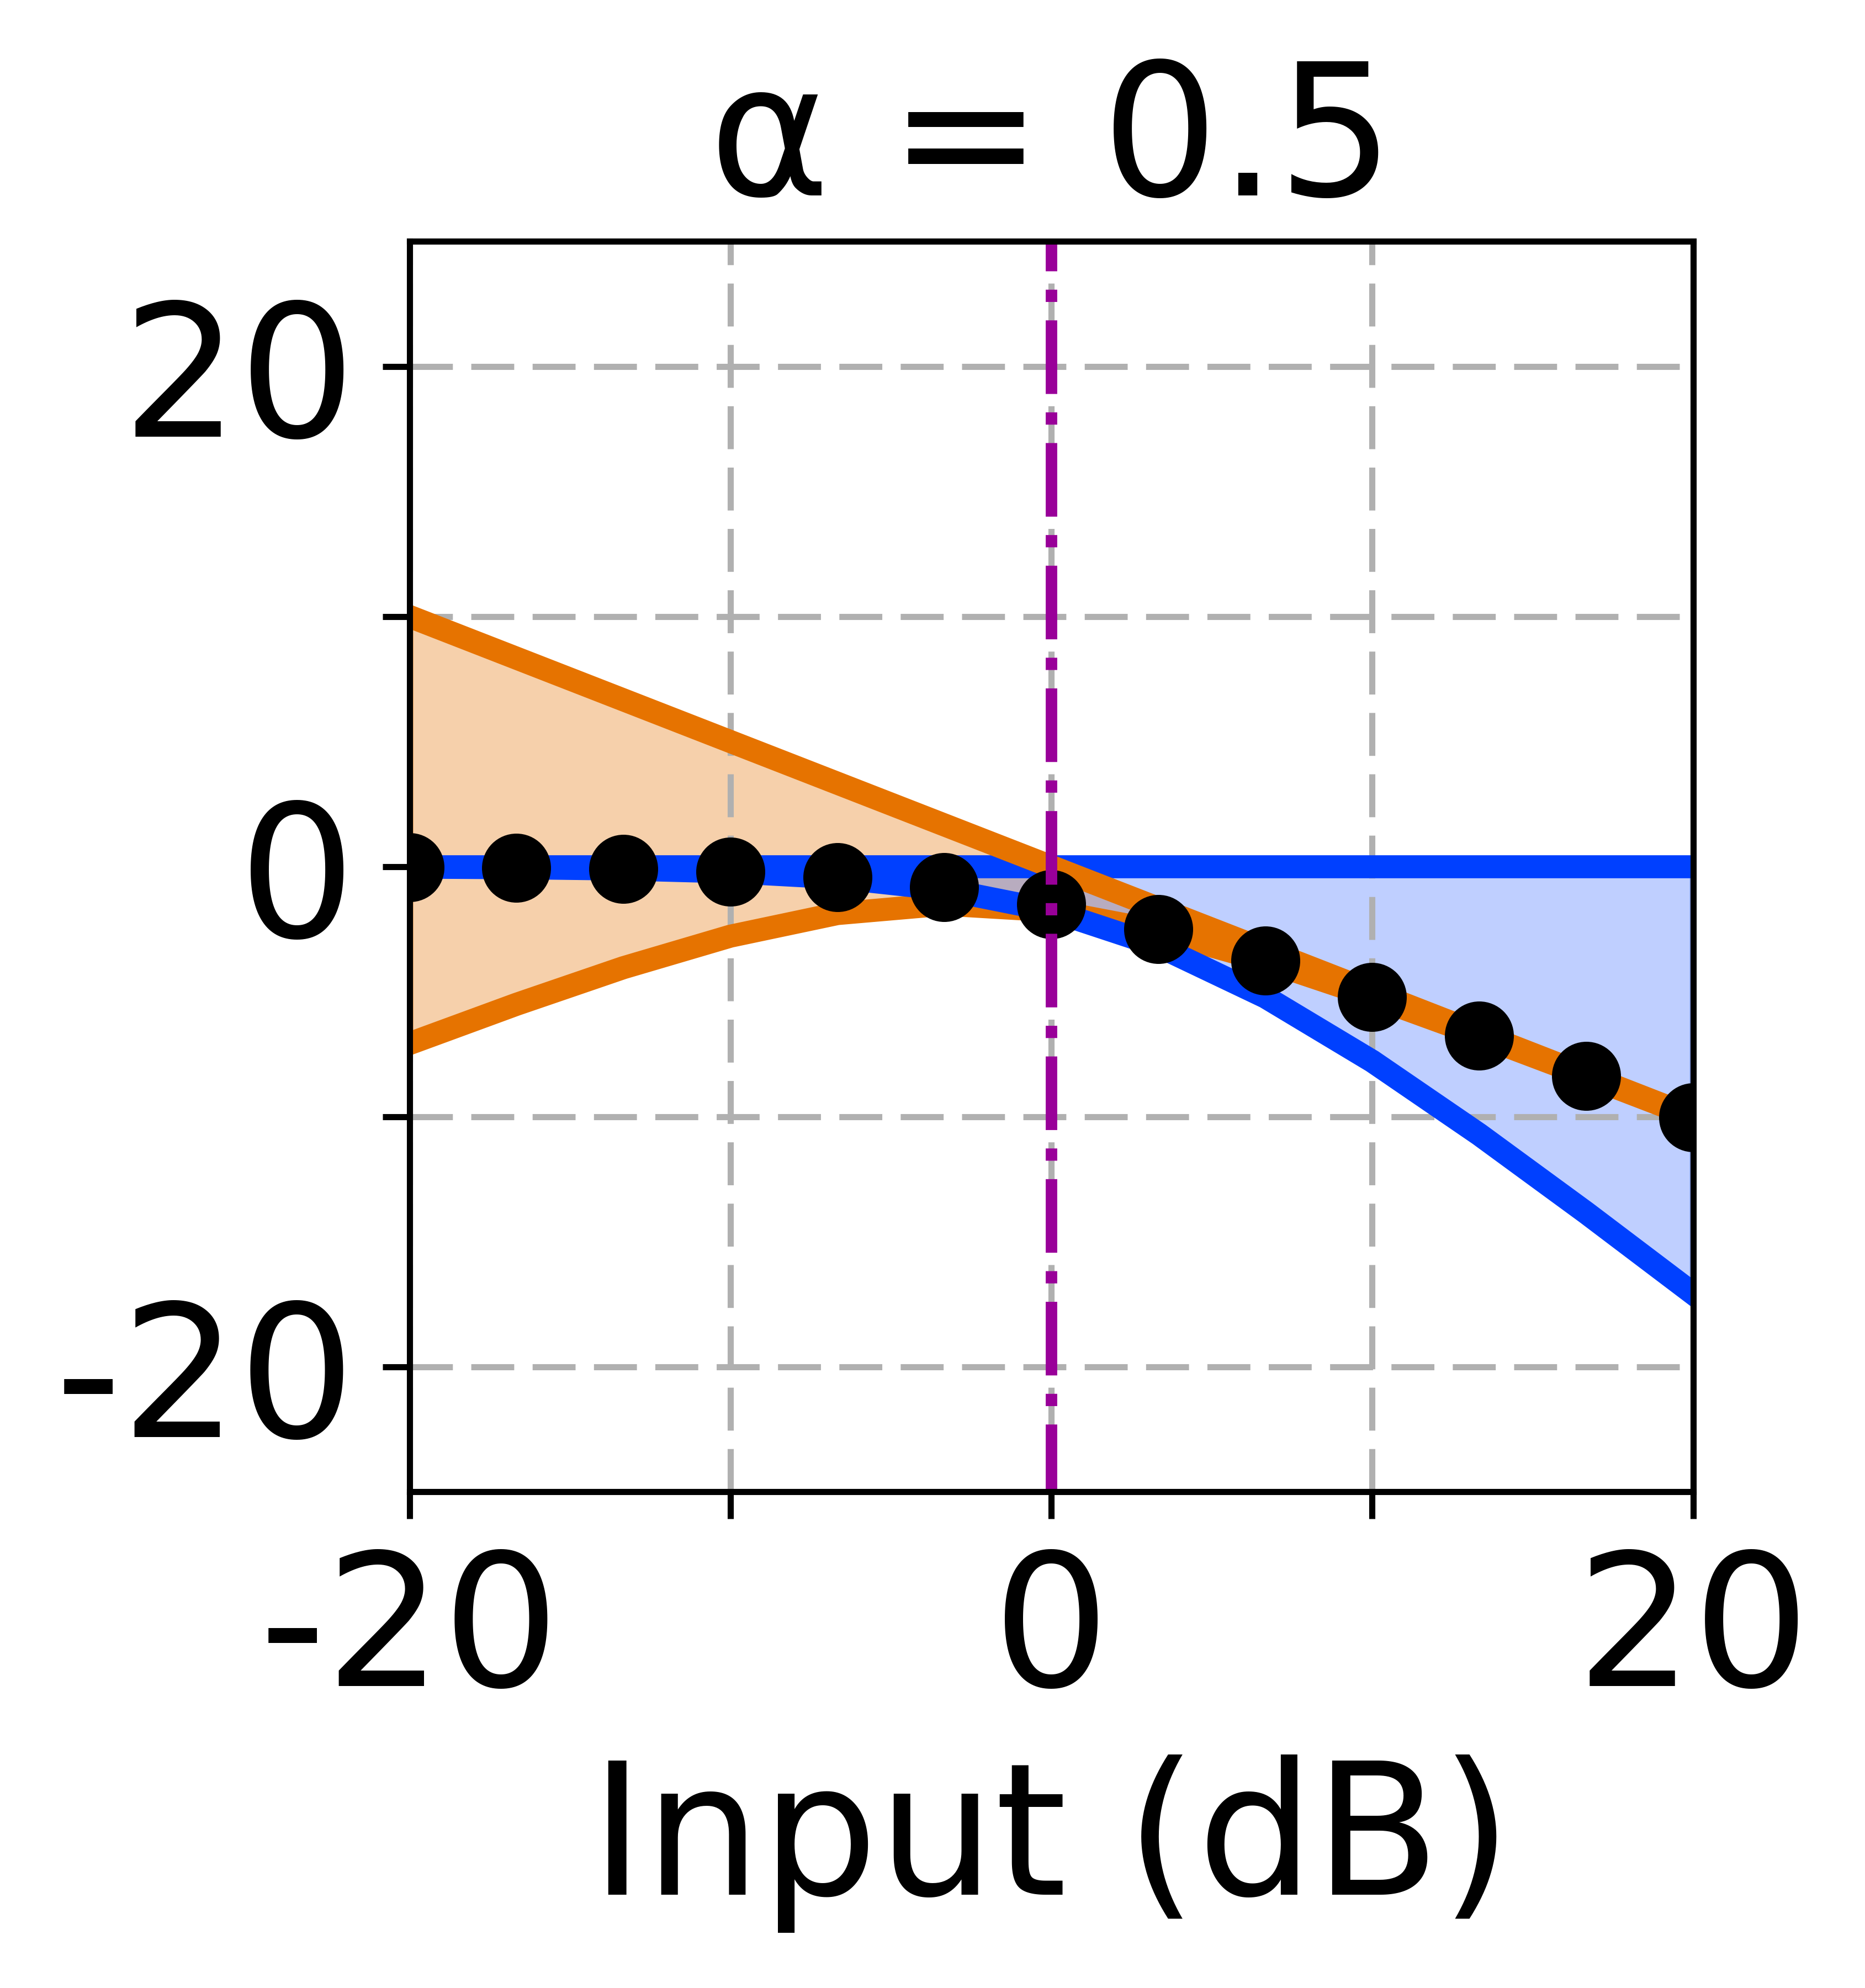
\includegraphics[height=0.33\linewidth]
{bode_renorm_0_5.png}
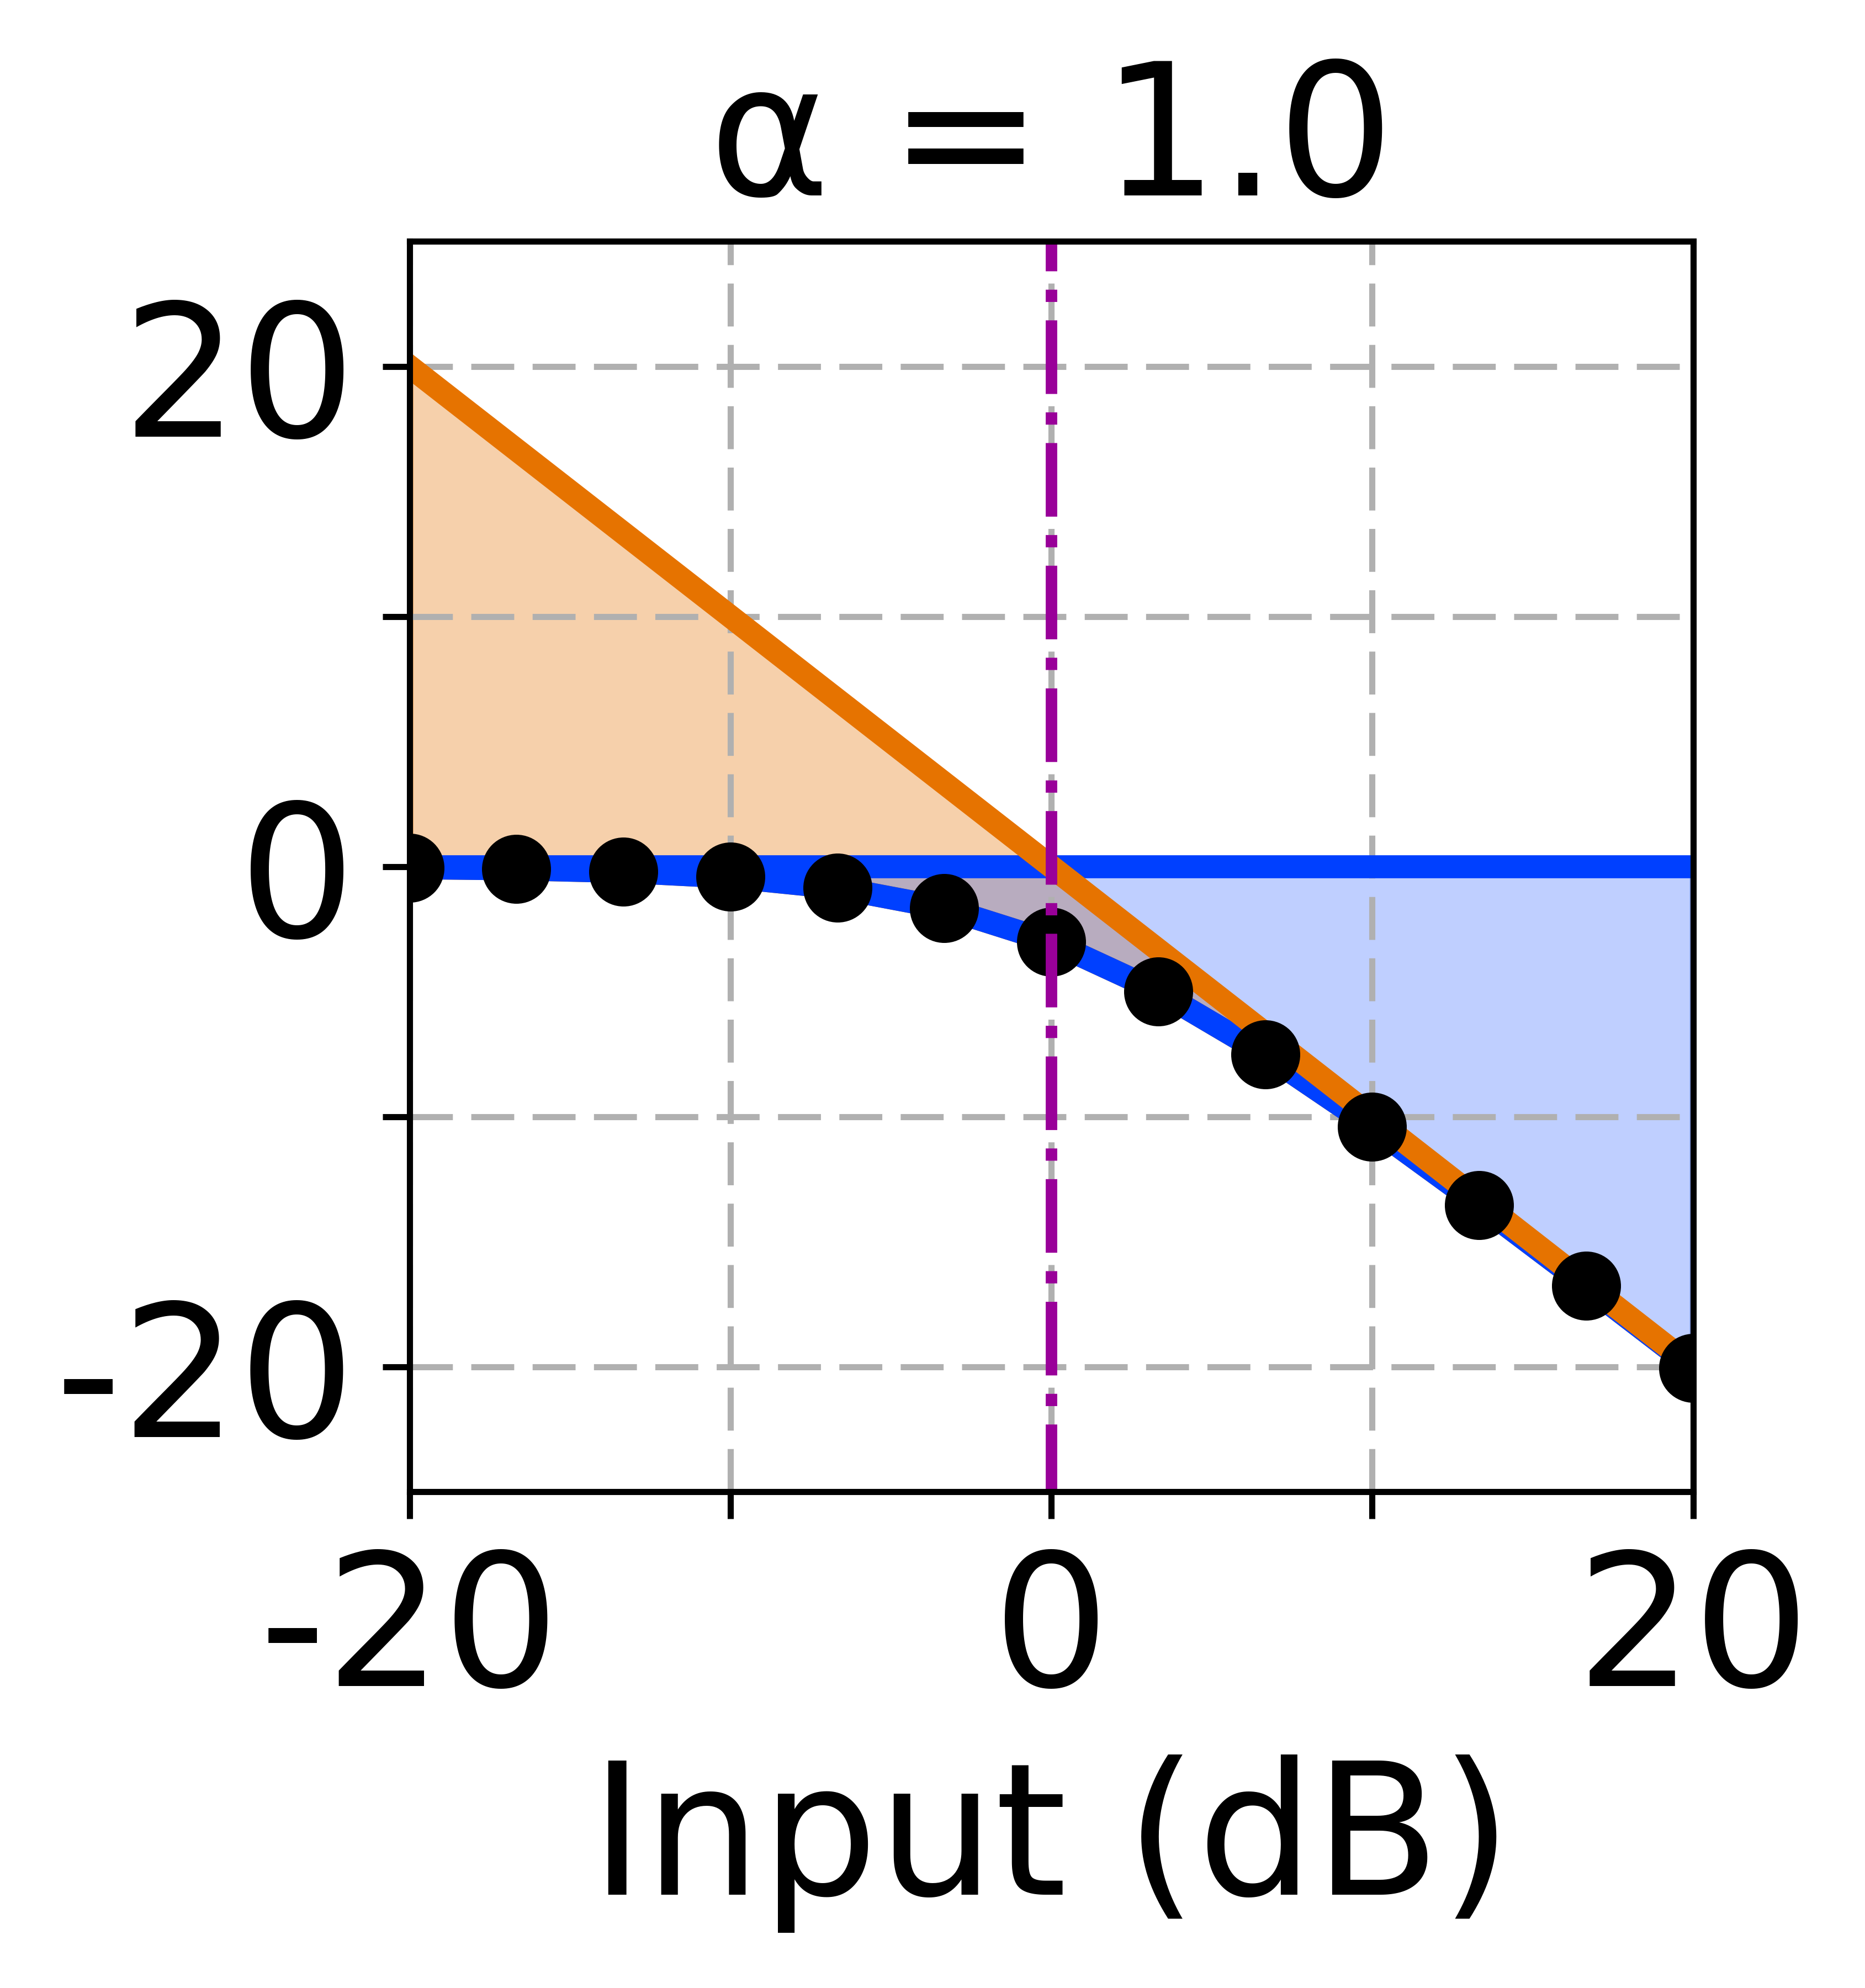
\includegraphics[height=0.33\linewidth]
{bode_renorm_1_0.png}

\includegraphics[height=0.5cm]
{bode_compressor_legend.png}
\caption{Static compression characteristic of gain $\mathbf{M} \mapsto (\varepsilon + \mathbf{M})^{-\alpha}$, as a function of the ratio $\frac{\mathbf{M}}{\varepsilon}$ between input magnitude $\mathbf{M}$ and soft threshold $\varepsilon$.
The exponent $\alpha$ is alternatively set to $0.1$ (left), $0.5$ (middle), and $1.0$ (right).
Solid lines and shaded areas respectively denote asymptotic bounds and their corresponding error margins, as proved in Proposition \ref{prop:gain-control}.
The dashed purple vertical line denotes the transition $\mathbf{M} = \varepsilon$.}
\label{fig:gain-control}
\end{figure}

\subsection{Dynamic range compression (DRC)}
The last stage of PCEN is the addition of a positive bias $\delta$ to $\mathbf{G}(t,f)$, followed by pointwise exponentiation of the sum:
\begin{align}
\mathbf{PCEN}(t,f) = &
(\mathbf{G}(t,f) + \delta)^r - \delta^r,
%\\ = &
%\left(\dfrac{\mathbf{E}(t,f)}{(\mathbf{M}(t,f)+\varepsilon)^\alpha}+ \delta \right)^r- \delta^r
\end{align}
where $0 < r < 1$ (\resp{} $\delta > 1$) is the exponent (\resp{} soft threshold) of dynamic range compression.

The parameter $\delta$ distinguishes two regimes: quiet ($\mathbf{G}\ll\delta$) and loud ($\mathbf{G}\gg\delta$) after AGC.
For $\mathbf{M}(t,f)\gg\varepsilon$, multiplying $\mathbf{E}(t,f)$ by some constant $C$ leads to $\mathbf{G}(t,f)$ being multiplied by $C^{1-\alpha}$ in the quiet regime, and by $C^{r(1-\alpha)}$ in the loud regime.
Therefore, DRC is stronger for smaller values of $r$.

\begin{prop}
$\mathbf{PCEN}$ is asymptotically equivalent to: (i) $r \delta^{(r-1)} \mathbf{G}$ for $\mathbf{G} \ll \delta$ and to (ii) $\mathbf{G}^r$ for $\mathbf{G} \gg \delta$.
\label{prop:loudness-compression}
\end{prop}

\begin{figure}
\centering
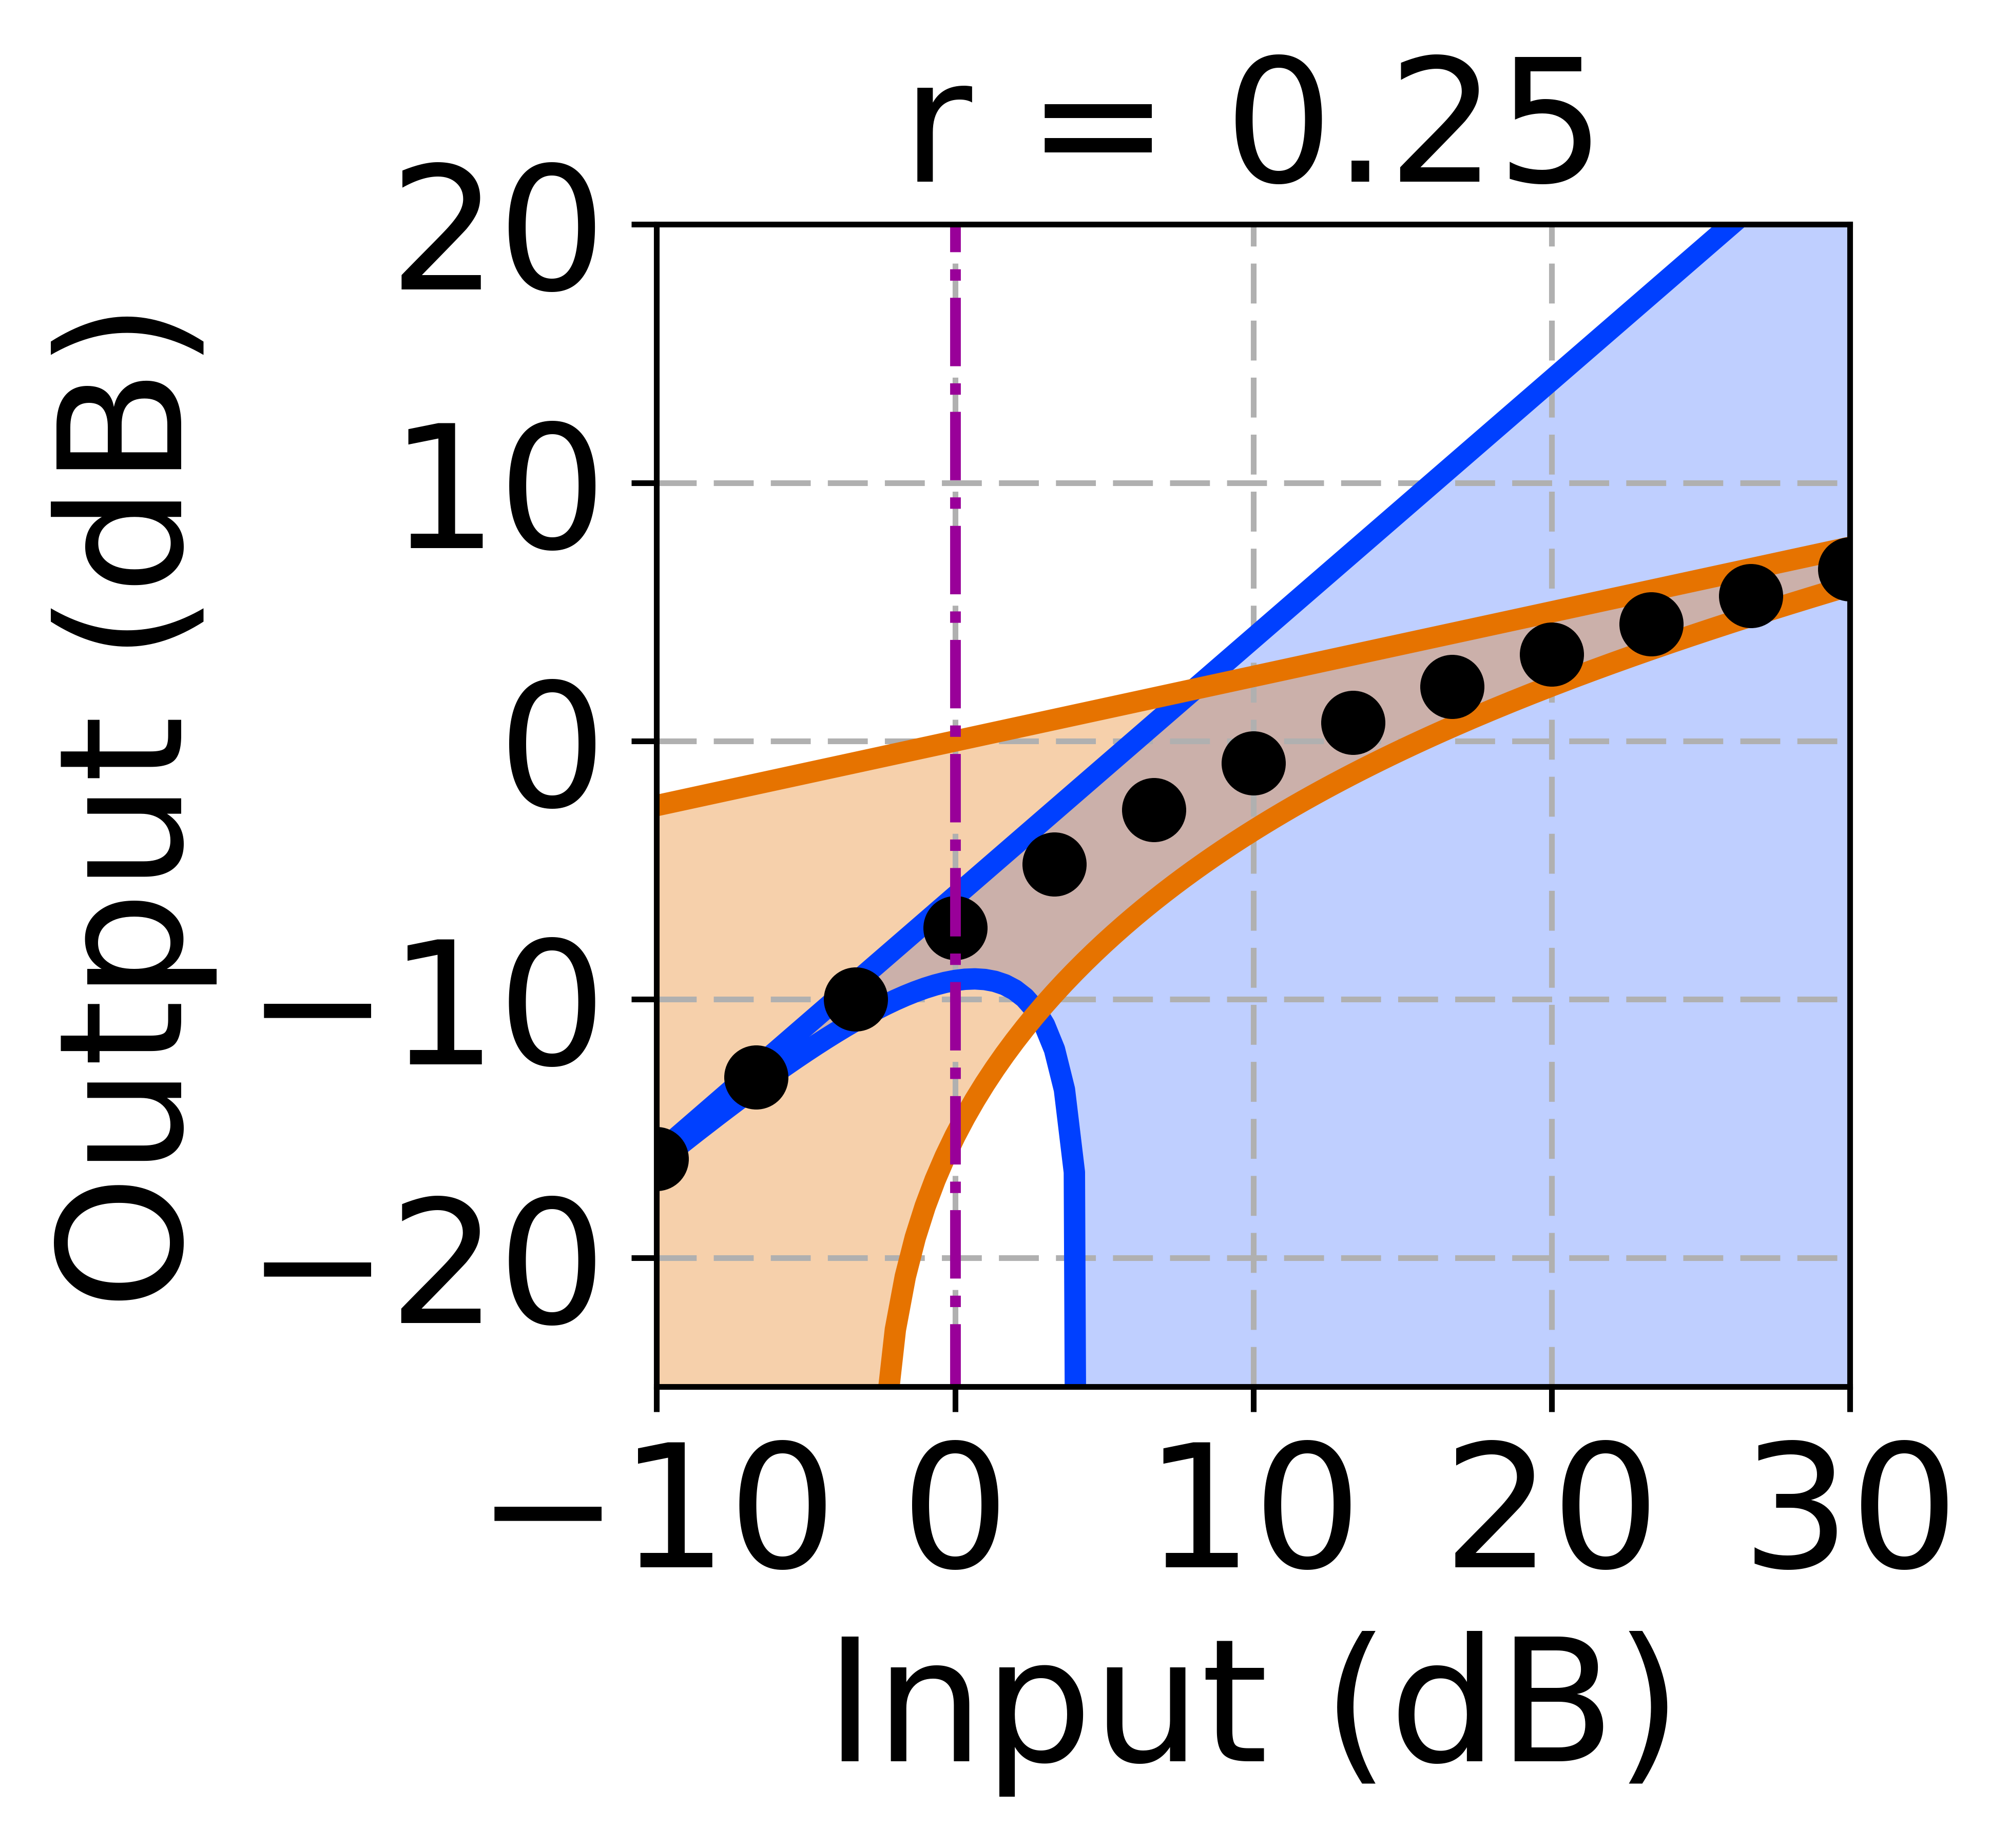
\includegraphics[height=0.33\linewidth]{bode_compressor_0_2.png}
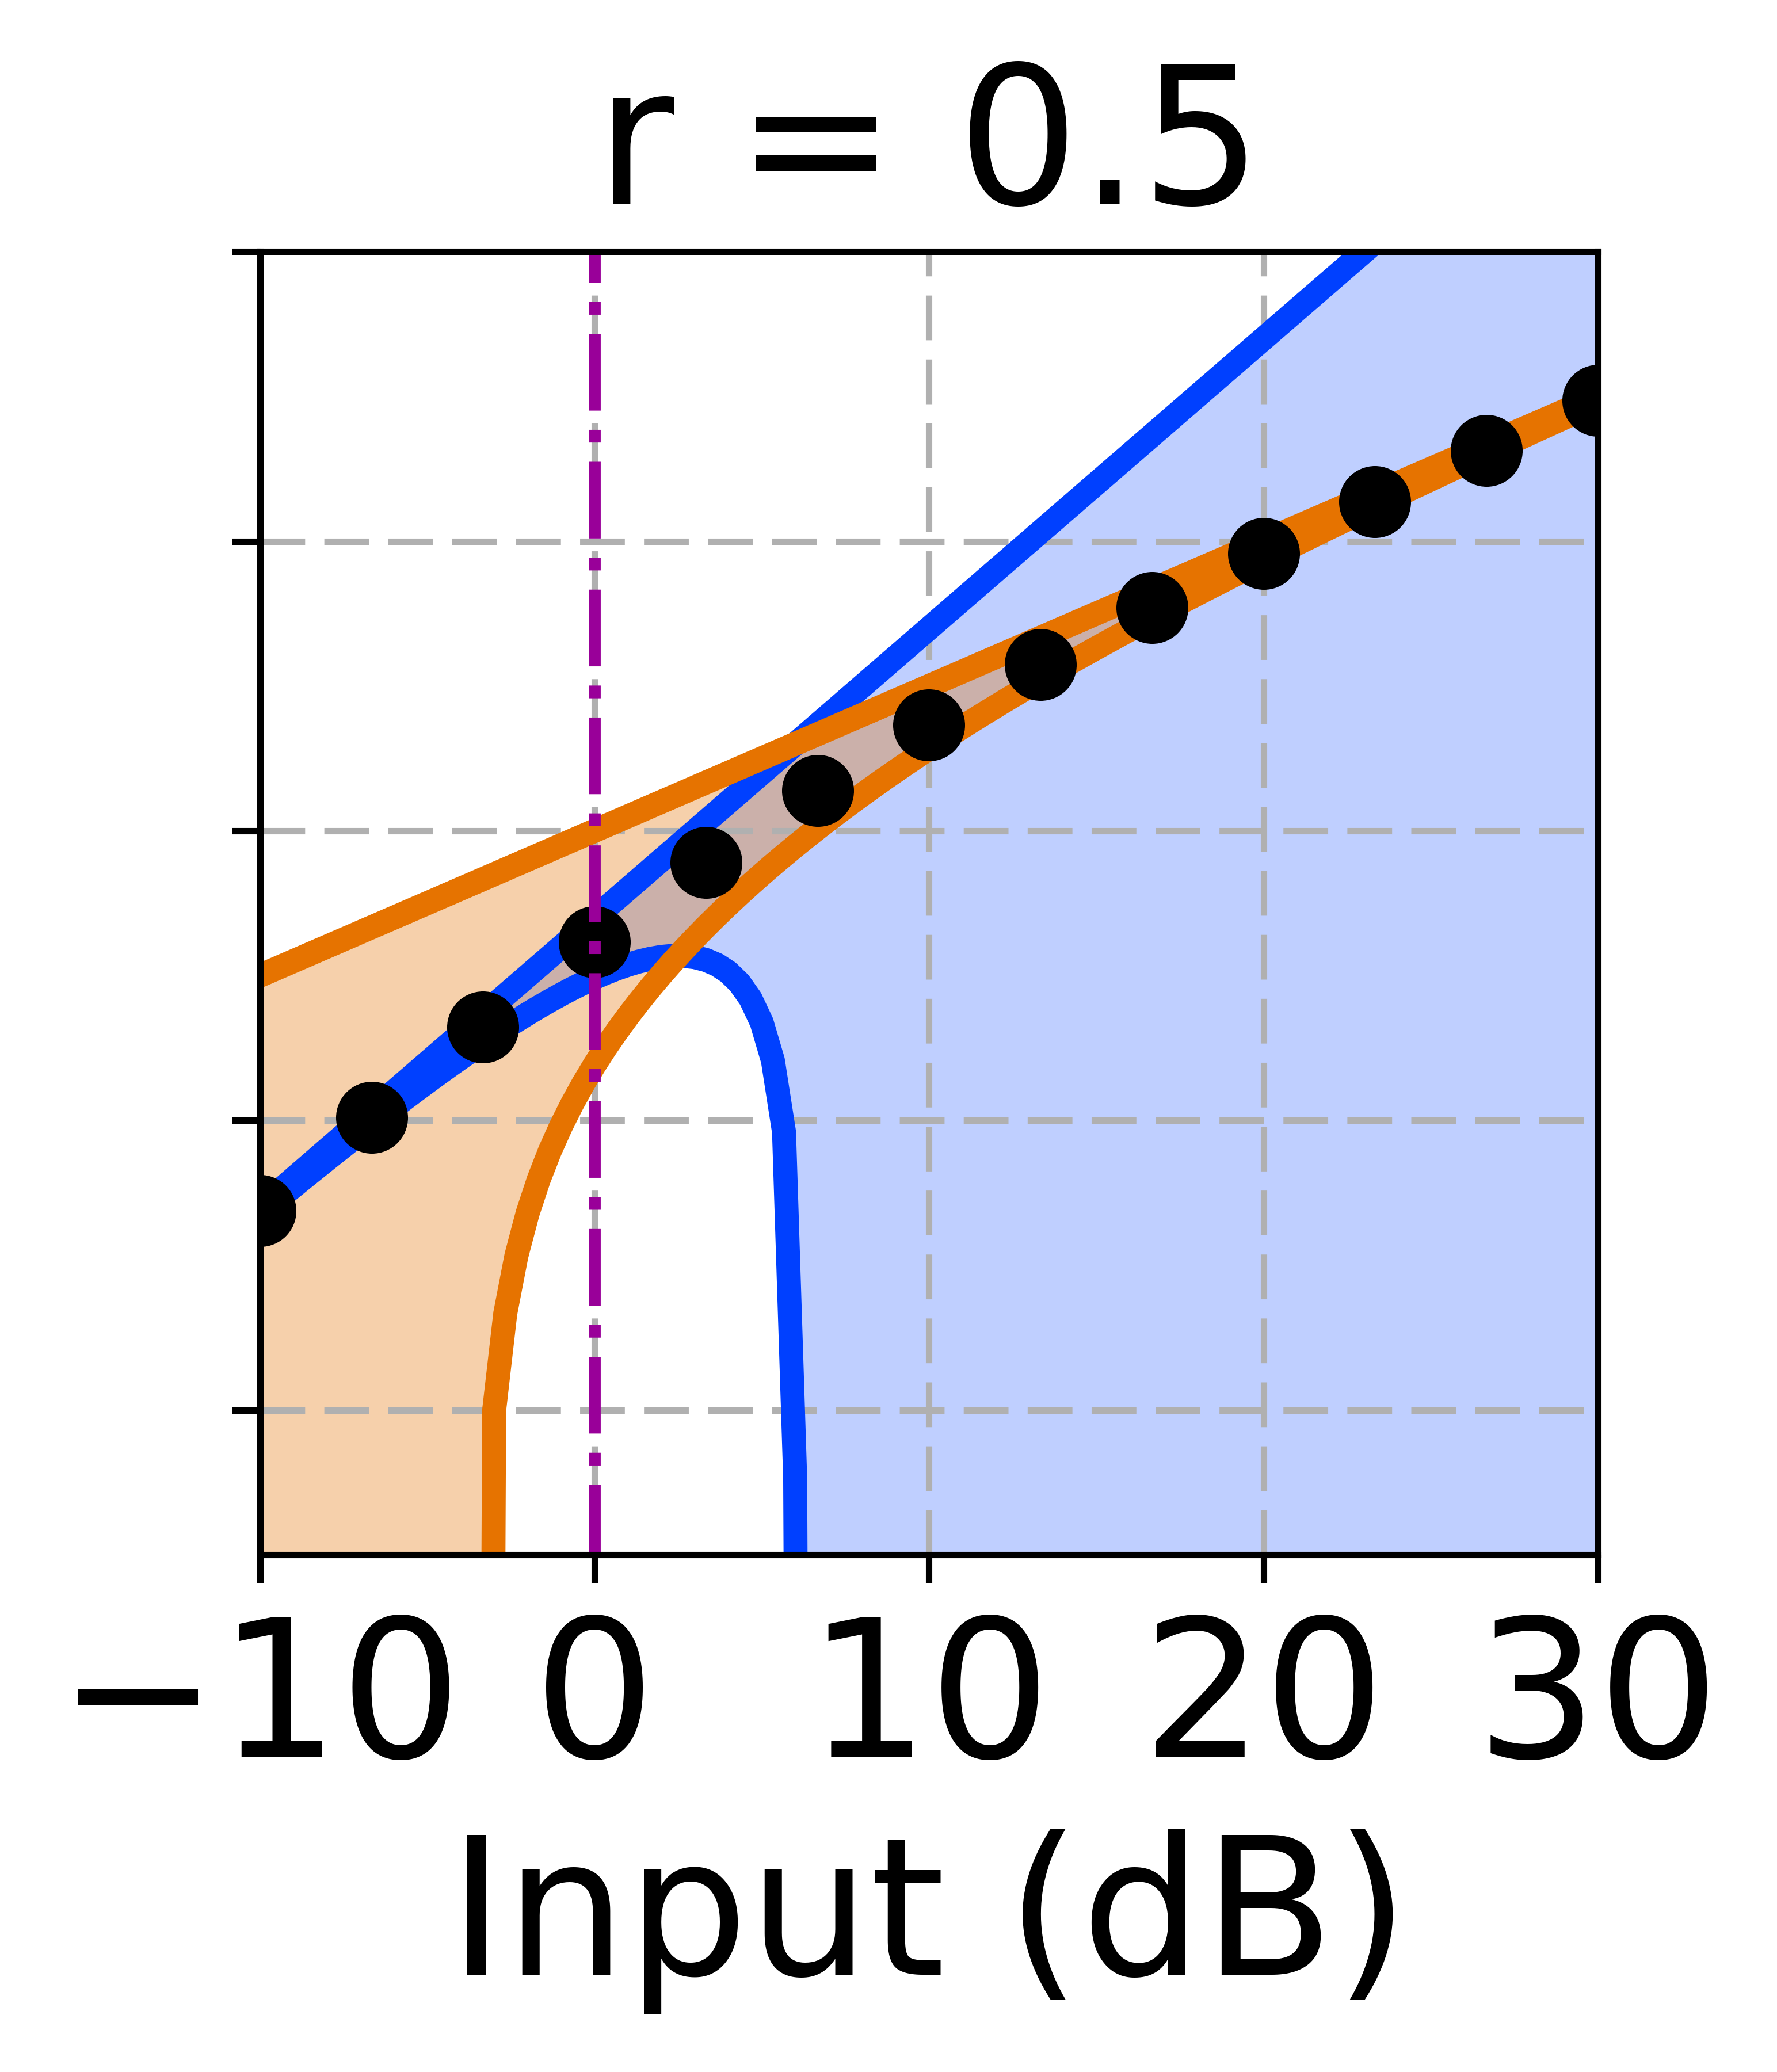
\includegraphics[height=0.33\linewidth]{bode_compressor_0_5.png}
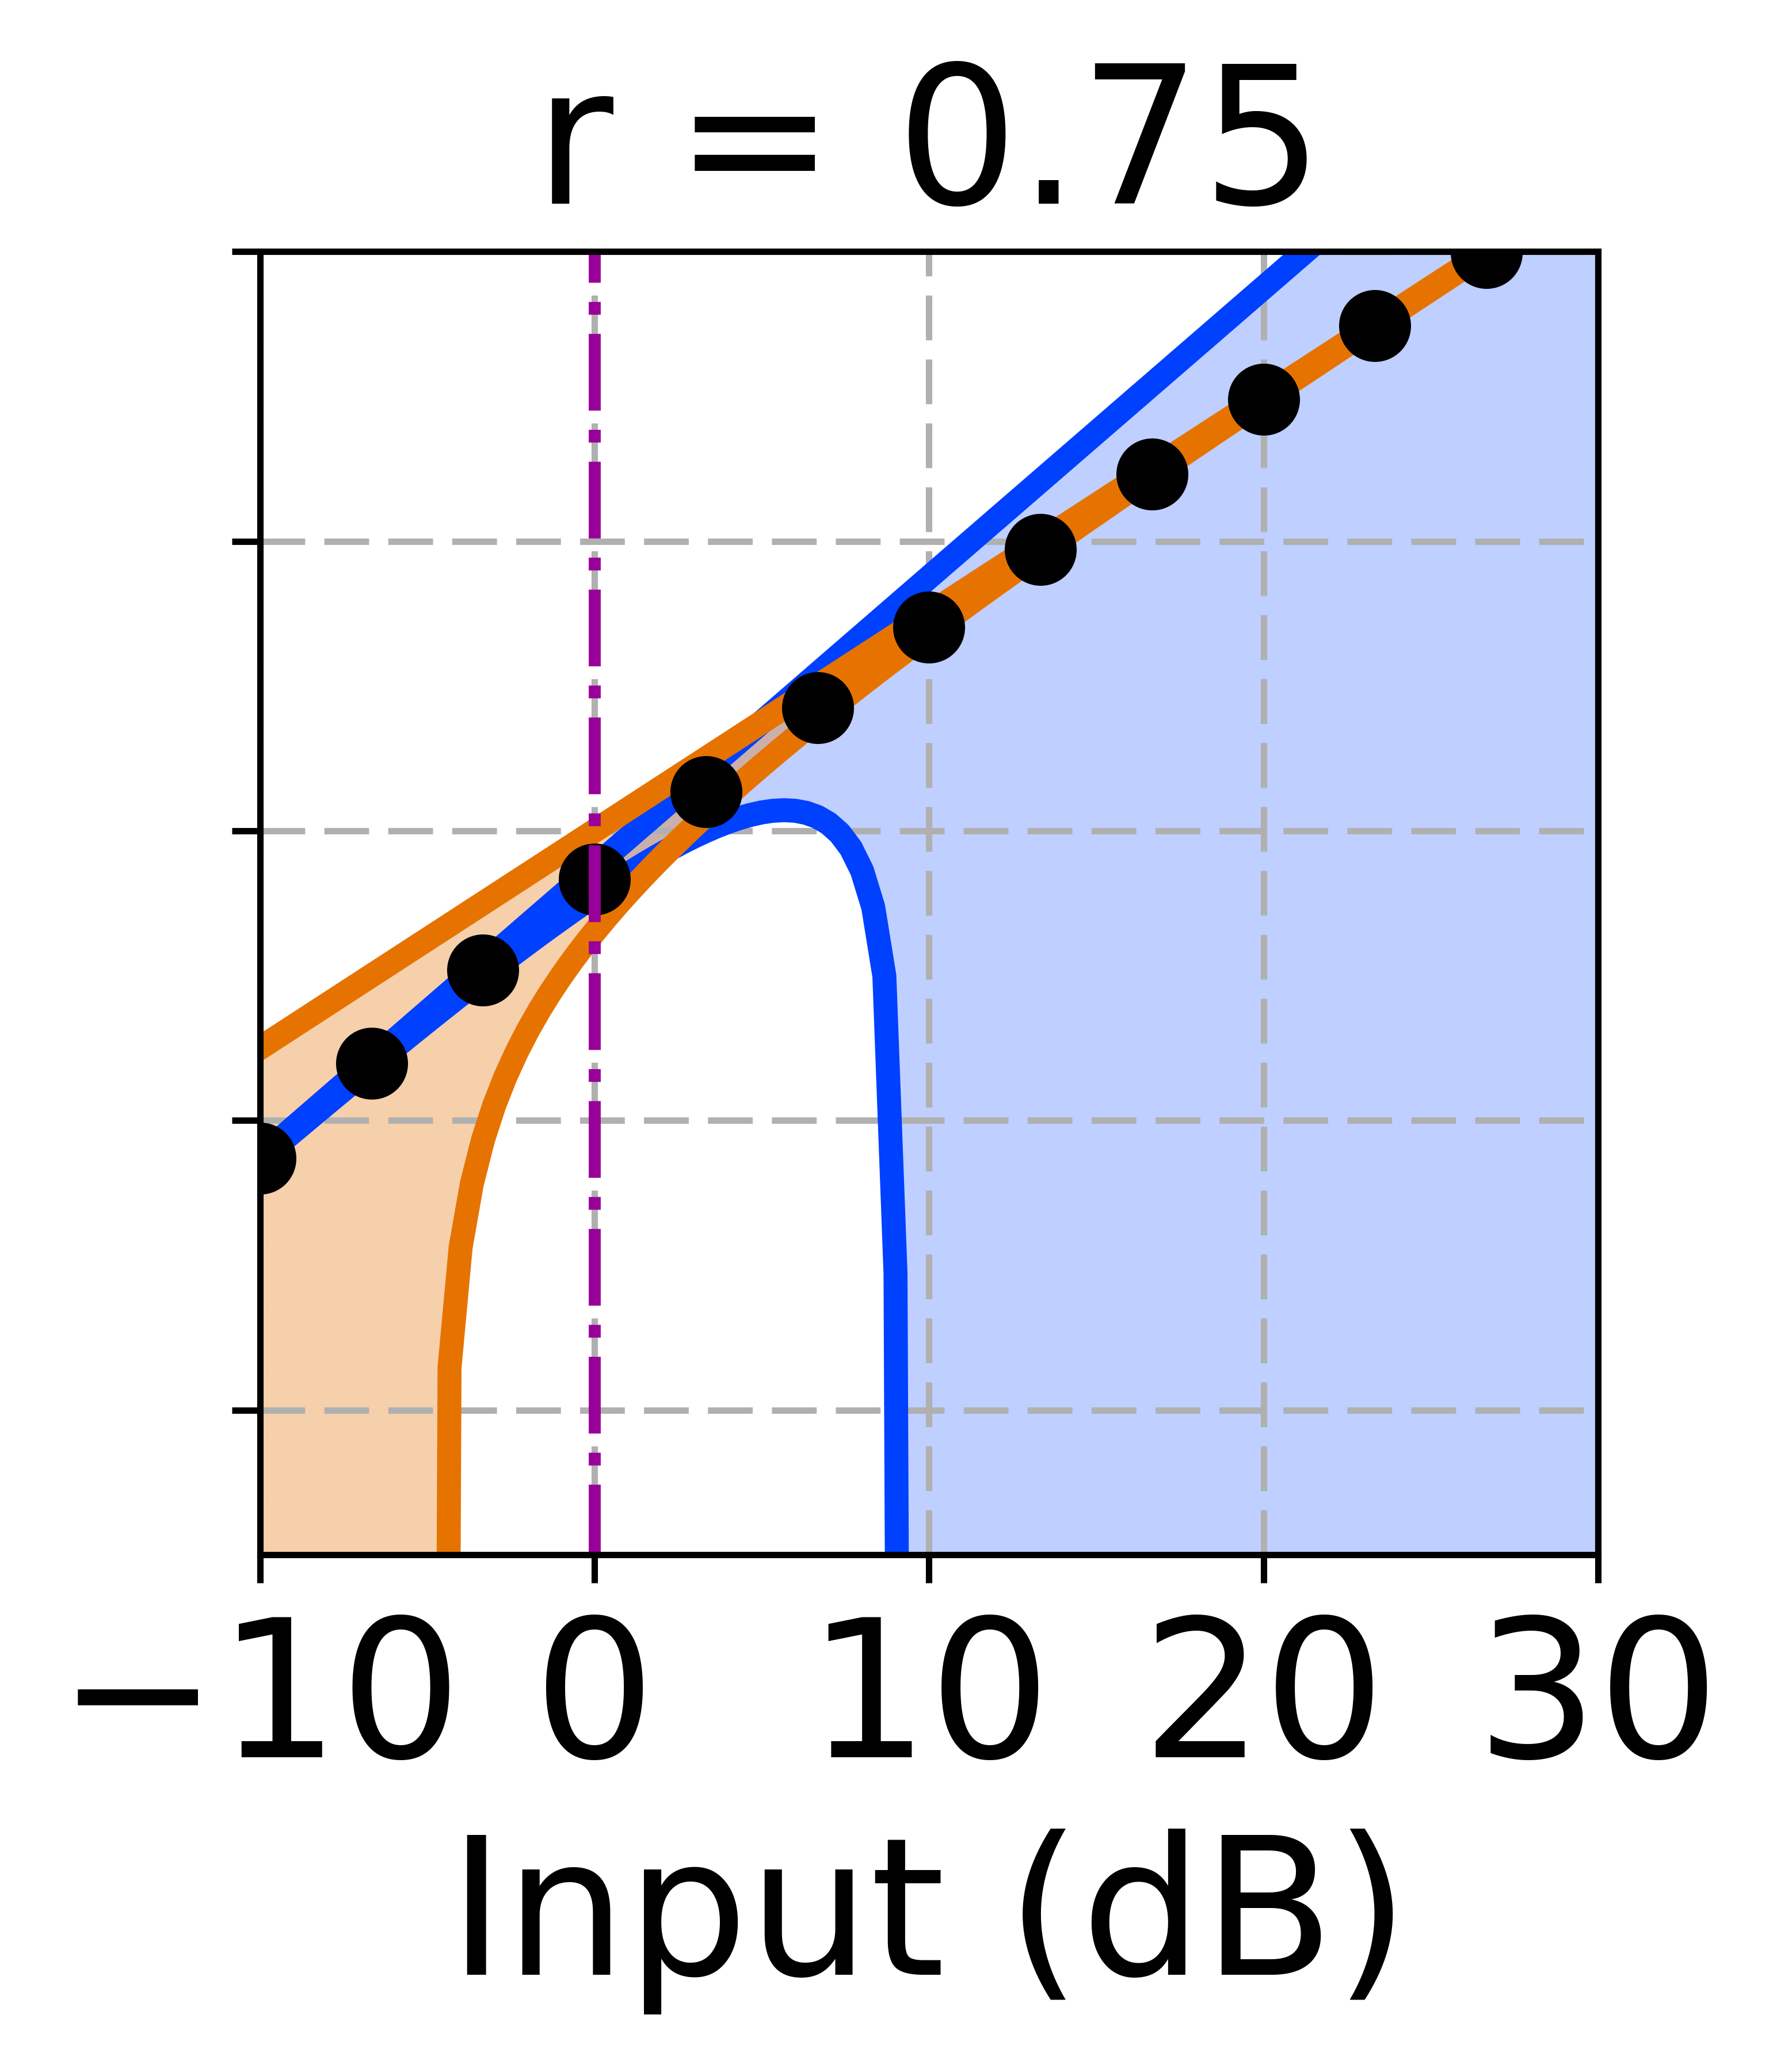
\includegraphics[height=0.33\linewidth]{bode_compressor_0_8.png}

\includegraphics[height=0.5cm]
{bode_compressor_legend.png}
\caption{Static compression characteristic of dynamic range compressions $\mathbf{G} \mapsto (\mathbf{G} + \delta)^r - \delta^r$, as a function of the ratio $\frac{\mathbf{G}}{\delta}$ between input magnitude $\mathbf{G}$ and soft threshold $\delta$,
for different values of $r$: $0.25$ (left), $0.5$ (right), and $0.75$ (right).
Solid lines and shaded areas respectively denote asymptotic bounds and their corresponding error margins, as proved in Proposition \ref{prop:loudness-compression}.}
\label{fig:loudness-compression}
\end{figure}

DRC resembles a spectral substraction in the context of speech restoration \cite{porter1984optimal}.
Figure \ref{fig:loudness-compression} illustrates the empirical fit of the characteristic $\mathbf{G} \mapsto (\mathbf{G} + \delta)^r - \delta^r$ to the asymptotic regimes described in Proposition \ref{prop:loudness-compression}.


\section{Practical recommendations\label{sec:practical-recommendations}}
%In this section, we share empirical findings regarding the effect of each parameter on the distribution of magnitudes in the time-frequency domain.


\subsection{Setting parameters $T$ and $s$}

As discussed in Subsection \ref{sub:temporal-integration}, the time constant $T$ (directly linked to the dimensionless parameter $s$) should be longer than the time taken by a frequency-modulated foreground event to move from one subband $f$ to another, adjacent subband.
For a mel-frequency spectrogram of $N$ bands ranging between $\mathrm{mel}(f_{\min})$ and $\mathrm{mel}(f_{\max})$, a rule of thumb for PCEN in AED is
\begin{equation}
\dfrac{T\times c \times N}{\mathrm{mel}(f_{\max}) - \mathrm{mel}(f_{\min})} = K,
\label{eq:rule-of-thumb}
\end{equation}
where $c$ is the typical chirp rate of the event of interest, measured in mels per second; and $K$ is some constant, depending on the reverberation properties of the environment.
If the mel-frequency spectrogram is replaced by a constant-$Q$ transform, the rule of thumb simply becomes $T \times c \times Q = K$,
where $c$ (\resp{} $Q$) is measured in octaves (\resp{} octaves per second).
$K$ is of the order of $1$ in  dry environments 
%(\eg{} ASR in the smart home \cite{lecouteux2011interspeech})
and above $10$ in highly reverberant environment, \eg{} bioacoustic event detection \cite{salamon2016plos,shonfield2017ace}.

In Equation \ref{eq:rule-of-thumb}, the optimal value of $T$ does not solely depend on the physical phenomenon of interest (through the chirp rate $c$ and reverberation constant $K$), but also on the choice of parametrization of the mel-frequency spectrogram (through $N$, $f_\mathrm{\min}$, and $f_\mathrm{\max}$).
Therefore,
in the context of hyperparameter optimization,
any change in the resolution of the time-frequency representation
%-- either mel-frequency spectrogram or CQT --
should be reflected in an update of $T$, which in turn updates $s$ through the following formula.
\begin{prop}
\label{prop:T-to-s}
%Let $T>0$ be some time scale for temporal integration.
At a discrete rate $\tau^{-1}$, the weight $s$ of the autoregressive filter $\boldsymbol{\phi}_T$ defined in Equation \ref{eq:autoregressive} is
\begin{equation}
s = \sqrt{1 - \cos \dfrac{2\pi \tau}{T}} \left(\sqrt{3 - \cos \dfrac{2\pi \tau}{T}} - \sqrt{1 - \cos \dfrac{2\pi \tau}{T}}  \right).
\end{equation}
\end{prop}

%For instance, the BirdVoxDetect system identifies avian flight calls such that $c \sim 6$ octaves per second by means of a mel-frequency spectrogram whose parameters are: $f_{\min} = \SI{2}{\kilo\hertz}$, $f_{\max} = \SI{10}{\kilo\hertz}$, $\tau = \SI{1.5}{\milli\second}$, and $N_\mathrm{mels} = 128$, \cite{lostanlen2017icassp}. We found the value $T = \SI{60}{\milli\second}$, \ie{} $s = 0.025$, to work well in practice.

\subsection{Setting parameters $\varepsilon$ and $\alpha$}

In accordance with \cite{wang2017icassp}, we found empirically that $T$ and $\alpha$ were the most important parameters.
Although $\alpha=1$ leads to an optimal cancellation of stationary background (see Prop. \ref{prop:invariance}), it may skew the distribution of magnitudes towards the right.
Setting $\alpha$ below $1$ reduces skewness and brings the background closer to AWGN.
However, we have found $\varepsilon$ to have no effect as long as it is set below unit roundoff.
%Thus, the main role of $\varepsilon$ is to avoid divisions by zero in the case of corrupted frequency bands.


\subsection{Setting parameters $\delta$ and $r$}

The effects of $\delta$ and $r$ are more noticeable on the foreground time-frequency regions than on the background.
The DRC threshold $\delta>1$ sets a tradeoff between improving average foreground-to-background ratio ($\delta\rightarrow+\infty$ in highly noisy applications) and reducing variance in the loudness of foreground events ($\delta\rightarrow1$).
Moreover, if the foreground source is transient with respect to the time scale $T$ and at distance $d$ from the sensor, the energy in $\mathbf{E}(t,f)$ is proportional to $\frac{1}{d^2}$: therefore, under a fixed background noise level $\mathbf{M}(t,f)$, one has $\mathbf{G}\sim\frac{1}{d^2}$ and $\mathbf{PCEN}\sim\frac{1}{d^{2r}}$.
We recommend $r=\frac{1}{2}$ for indoor applications ($d\sim\SI{10}{\meter}$) and $r=\frac{1}{4}$ for outdoor applications ($d\sim\SI{100}{\meter}$).


\subsection{Open source implementation of PCEN in librosa}
We release an open source implementation of PCEN in librosa v0.6.1 \cite{mcfee2018librosa061}, whose default parameters are identical to \cite{wang2017icassp}:  $T=\SI{400}{\milli\second}$ (\ie{} $s\approx0.025$ with $\tau = \SI{23}{\milli\second}$), $\varepsilon=10^{-6}$, $\alpha=0.98$, $\delta=2$, and $r=\frac{1}{2}$.
Whereas these defaults are best suited to indoor applications (\eg{} ASR in the smart home), bioacoustic event detection distinguishes itself by faster modulations of foreground (lower $T$), higher skewness of background magnitudes (lower $\alpha$), a louder background (higher $\delta$), and more distant sources (lower $r$).
Thus, we adopt the following settings in our bird detection work: $T=\SI{60}{\milli\second}$ with $Q=50$ and $\tau=\SI{1.5}{\milli\second}$, $\varepsilon=10^{-6}$, $\alpha=0.8$, $\delta=10$, and $r=0.25$.
The inspection of magnitude histograms (Figure \ref{fig:gaussianization}) and covariance matrices (Figure \ref{fig:decorrelation}) suggests that such settings lead to a successful Gaussianization and decorrelation of subbands.

\section{Conclusion}
%The human auditory system exhibits a remarkable ability to identify cues from distant sources, despite the presence of environmental absorption, reverberation, and noise \cite{meyer2013plos}.
%At the level of the cochlea, two factors explaining such ability are:
%the band-pass frequential selectivity of inner hair cell stereocilia, known as tonotopy;
%and the loudness adaptation of outer hair cells, known as electromotility \cite{robles2001physiolrev}.
%While the mel scale simulates tonotopy \cite{kaya2017philtrans}, PCEN simulates electromotility: as we have found empirically, it Gaussianizes real-world background noise, in real time, at a modest computational cost.

Unlike batch learning decorrelation procedures such as principal component analysis (PCA), PCEN can be implemented in real time and distributed across sensors \cite{bello2018cacm}; in addition, it preserves the locality structure of harmonic patterns along the mel-frequency axis \cite{lostanlen2016ismir}.
Although it depends on five parameters ($T$, $\alpha$, $\varepsilon$, $r$, and $\delta$) that are possibly frequency-dependent, this article has shown that each of these parameters has an interpretable purpose, and given asymptotic approximations of the PCEN equations in ideal regimes: silent \vs{} active ($\varepsilon$), stationary \vs{} transient ($T$), and quiet \vs{} loud ($\delta$).
In the context of deep learning for ASR and AED, our results could yield well-adapted initial values for the trainable version of PCEN \cite{wang2017icassp}, as well as a post hoc interpretation of all learned parameters.

% use section* for acknowledgment
\section*{Acknowledgment}
The authors wish to thank Richard F. Lyon for helpful discussions.
This work is partially supported by NSF awards 1633206 and 1633259, the
Leon Levy Foundation, and a Google faculty award.


% Can use something like this to put references on a page
% by themselves when using endfloat and the captionsoff option.
%\ifCLASSOPTIONcaptionsoff
%  \newpage
%\fi
%\newpage


% trigger a \newpage just before the given reference
% number - used to balance the columns on the last page
% adjust value as needed - may need to be readjusted if
% the document is modified later
%-\IEEEtriggeratref{8}
% The "triggered" command can be changed if desired:
%\IEEEtriggercmd{\enlargethispage{-5in}}

% references section

% can use a bibliography generated by BibTeX as a .bbl file
% BibTeX documentation can be easily obtained at:
% http://mirror.ctan.org/biblio/bibtex/contrib/doc/
% The IEEEtran BibTeX style support page is at:
% http://www.michaelshell.org/tex/ieeetran/bibtex/
\bibliographystyle{IEEEtran}
% argument is your BibTeX string definitions and bibliography database(s)
\bibliography{IEEEabrv,lostanlen2018spl}
%
% <OR> manually copy in the resultant .bbl file
% set second argument of \begin to the number of references
% (used to reserve space for the reference number labels box)
%\begin{thebibliography}{1}

%\bibitem{IEEEhowto:kopka}
%H.~Kopka and P.~W. Daly, \emph{A Guide to \LaTeX}, 3rd~ed.\hskip 1em plus
%  0.5em minus 0.4em\relax Harlow, England: Addison-Wesley, 1999.

%\end{thebibliography}

% biography section
% 
% If you have an EPS/PDF photo (graphicx package needed) extra braces are
% needed around the contents of the optional argument to biography to prevent
% the LaTeX parser from getting confused when it sees the complicated
% \includegraphics command within an optional argument. (You could create
% your own custom macro containing the \includegraphics command to make things
% simpler here.)
%\begin{IEEEbiography}[{\includegraphics[width=1in,height=1.25in,clip,keepaspectratio]{mshell}}]{Michael Shell}
% or if you just want to reserve a space for a photo:

%\begin{IEEEbiography}{Michael Shell}
%Biography text here.
%\end{IEEEbiography}

% if you will not have a photo at all:
%\begin{IEEEbiographynophoto}{John Doe}
%Biography text here.
%\end{IEEEbiographynophoto}

% insert where needed to balance the two columns on the last page with
% biographies
%\newpage

%\begin{IEEEbiographynophoto}{Jane Doe}
%Biography text here.
%\end{IEEEbiographynophoto}

% You can push biographies down or up by placing
% a \vfill before or after them. The appropriate
% use of \vfill depends on what kind of text is
% on the last page and whether or not the columns
% are being equalized.

%\vfill

% Can be used to pull up biographies so that the bottom of the last one
% is flush with the other column.
%\enlargethispage{-5in}



% that's all folks
\end{document}


% An example of a floating figure using the graphicx package.
% Note that \label must occur AFTER (or within) \caption.
% For figures, \caption should occur after the \includegraphics.
% Note that IEEEtran v1.7 and later has special internal code that
% is designed to preserve the operation of \label within \caption
% even when the captionsoff option is in effect. However, because
% of issues like this, it may be the safest practice to put all your
% \label just after \caption rather than within \caption{}.
%
% Reminder: the "draftcls" or "draftclsnofoot", not "draft", class
% option should be used if it is desired that the figures are to be
% displayed while in draft mode.
%
%\begin{figure}[!t]
%\centering
%\includegraphics[width=2.5in]{myfigure}
% where an .eps filename suffix will be assumed under latex, 
% and a .pdf suffix will be assumed for pdflatex; or what has been declared
% via \DeclareGraphicsExtensions.
%\caption{Simulation results for the network.}
%\label{fig_sim}
%\end{figure}

% Note that the IEEE typically puts floats only at the top, even when this
% results in a large percentage of a column being occupied by floats.


% An example of a double column floating figure using two subfigures.
% (The subfig.sty package must be loaded for this to work.)
% The subfigure \label commands are set within each subfloat command,
% and the \label for the overall figure must come after \caption.
% \hfil is used as a separator to get equal spacing.
% Watch out that the combined width of all the subfigures on a 
% line do not exceed the text width or a line break will occur.
%

%
% Note that often IEEE papers with subfigures do not employ subfigure
% captions (using the optional argument to \subfloat[]), but instead will
% reference/describe all of them (a), (b), etc., within the main caption.
% Be aware that for subfig.sty to generate the (a), (b), etc., subfigure
% labels, the optional argument to \subfloat must be present. If a
% subcaption is not desired, just leave its contents blank,
% e.g., \subfloat[].


% An example of a floating table. Note that, for IEEE style tables, the
% \caption command should come BEFORE the table and, given that table
% captions serve much like titles, are usually capitalized except for words
% such as a, an, and, as, at, but, by, for, in, nor, of, on, or, the, to
% and up, which are usually not capitalized unless they are the first or
% last word of the caption. Table text will default to \footnotesize as
% the IEEE normally uses this smaller font for tables.
% The \label must come after \caption as always.
%
%\begin{table}[!t]
%% increase table row spacing, adjust to taste
%\renewcommand{\arraystretch}{1.3}
% if using array.sty, it might be a good idea to tweak the value of
% \extrarowheight as needed to properly center the text within the cells
%\caption{An Example of a Table}
%\label{table_example}
%\centering
%% Some packages, such as MDW tools, offer better commands for making tables
%% than the plain LaTeX2e tabular which is used here.
%\begin{tabular}{|c||c|}
%\hline
%One & Two\\
%\hline
%Three & Four\\
%\hline
%\end{tabular}
%\end{table}


% Note that the IEEE does not put floats in the very first column
% - or typically anywhere on the first page for that matter. Also,
% in-text middle ("here") positioning is typically not used, but it
% is allowed and encouraged for Computer Society conferences (but
% not Computer Society journals). Most IEEE journals/conferences use
% top floats exclusively. 
% Note that, LaTeX2e, unlike IEEE journals/conferences, places
% footnotes above bottom floats. This can be corrected via the
% \fnbelowfloat command of the stfloats package.